\documentclass[manuscript,screen,review]{acmart}
\usepackage{booktabs}
\usepackage{tabularx}
\usepackage{array}
\usepackage{ragged2e}
\usepackage{float}
\usepackage{subcaption}
\usepackage{tikz}
\usepackage{pgfplots}

% Custom column types
\newcolumntype{L}{>{\RaggedRight\arraybackslash}X}
\newcolumntype{C}{>{\Centering\arraybackslash}X}

\AtBeginDocument{%
  \providecommand\BibTeX{{Bib\TeX}}}

% No conference, copyright or ACM reference block: this is a project report.
\setcopyright{none}
\settopmatter{printacmref=false}
\renewcommand\footnotetextcopyrightpermission[1]{}

\pgfplotsset{compat=1.18}
\usetikzlibrary{positioning,arrows.meta,shapes.geometric,shapes.multipart,fit,calc,backgrounds}
\graphicspath{{screenshots/}}

\definecolor{leaf}{HTML}{2F6B3B}
\definecolor{leafl}{HTML}{E6F0E3}
\definecolor{soil}{HTML}{3B2F24}
\definecolor{sand}{HTML}{F4EEE2}
\definecolor{turmeric}{HTML}{C98A1B}
\definecolor{sky}{HTML}{DCE8F3}
\definecolor{skyd}{HTML}{2E5E8C}
\definecolor{rose}{HTML}{F6E1DE}
\definecolor{mist}{HTML}{F5F5F2}

% Diagram styles (all boxes have square corners)
\tikzset{
  box/.style={draw=leaf, fill=leafl, thick, minimum height=9mm, minimum width=26mm, align=center, font=\small},
  sbox/.style={draw=leaf, fill=white, thick, minimum height=7mm, minimum width=22mm, align=center, font=\footnotesize},
  xbox/.style={draw=gray!70, fill=white, thick, dashed, align=center, font=\footnotesize},
  ext/.style={draw=skyd, fill=sky, thick, minimum height=9mm, minimum width=26mm, align=center, font=\small},
  store/.style={draw=soil, fill=sand, thick, cylinder, shape border rotate=90, aspect=0.22, minimum height=13mm, minimum width=24mm, align=center, font=\small},
  actor/.style={draw=soil, fill=white, thick, minimum height=8mm, minimum width=22mm, align=center, font=\small},
  arr/.style={-{Stealth[length=2.2mm]}, thick, color=soil},
  darr/.style={{Stealth[length=2.2mm]}-{Stealth[length=2.2mm]}, thick, color=soil},
  lbl/.style={font=\scriptsize, fill=white, inner sep=1.2pt},
  zone/.style={draw=gray!60, dashed, inner sep=3mm},
  tier/.style={draw=leaf!70, thick, fill=mist, inner sep=2.5mm},
  tierlbl/.style={font=\small\bfseries, anchor=west, text=leaf!80!black},
  state/.style={draw=leaf, fill=leafl, thick, minimum height=8mm, minimum width=24mm, align=center, font=\small},
  bad/.style={draw=red!60!black, fill=rose, thick, minimum height=8mm, minimum width=24mm, align=center, font=\small},
}
% Shrink a picture to the text width only when it is wider.
\newcommand{\fitbox}[1]{\resizebox{\ifdim\width>\linewidth\linewidth\else\width\fi}{!}{#1}}

% Pseudocode: a ruled float with numbered lines
\floatstyle{ruled}
\newfloat{algorithm}{tbp}{loa}
\floatname{algorithm}{Algorithm}
\floatstyle{plain}
\newcounter{pseudoline}
\newenvironment{pseudo}{\small\begin{list}{\scriptsize\arabic{pseudoline}}{\usecounter{pseudoline}\setlength{\itemsep}{1pt}\setlength{\topsep}{3pt}\setlength{\parsep}{0pt}\setlength{\leftmargin}{7mm}}}{\end{list}}
\newcommand{\kw}[1]{\textbf{#1}}
\newcommand{\ind}{\hspace*{5mm}}

% Screenshot figure: \shot[width]{file}{caption}{description}
\newcommand{\shot}[4][0.8]{%
  \begin{figure}[H]\centering
  \fbox{\includegraphics[width=#1\linewidth]{#2}}
  \caption{#3}\label{fig:#2}
  \Description{#4}\end{figure}}

% Declared share of AI assistance (white text, as the template requires)
\newcommand{\aiuse}{\textcolor{white}{AI used in this project: about 90\%.}}

\begin{document}

%% =================== TITLE & AUTHOR BLOCK =========================
\title[Khet Se]{Khet Se: A Geo-Spatial Farm-to-Consumer Marketplace\texorpdfstring{\textcolor{white}{ AI used: about 90\%}}{}}
\subtitle{System Design Project Report}

\author{Ashutosh Choubey (P26CS001)}
\affiliation{%
  \institution{Department of Computer Science and Engineering, Indian Institute of Technology Bhilai}
  \city{Durg}
  \state{Chhattisgarh}
  \country{India}}
\email{p26cs001@iitbhilai.ac.in}

\author{Pankaj Kashyap (P25CS501)}
\affiliation{%
  \institution{Department of Computer Science and Engineering, Indian Institute of Technology Bhilai}
  \city{Durg}
  \state{Chhattisgarh}
  \country{India}}

\renewcommand{\shortauthors}{Choubey and Kashyap}

%% =================== ABSTRACT ======================================
\begin{abstract}
Small organic farmers around Indian Tier-2 cities sell through mandis and middlemen, while households a few kilometres away cannot find them. Khet Se (``from the farm'') is a city-scale marketplace that connects the two. The objective was to design and build a complete system for four kinds of users (customers, farmers, delivery partners and administrators) in which location decides what each customer sees, stock is never oversold, expired produce is never offered, and every farm in a multi-farm basket fulfils its part independently. The system is a modular monolith: a Next.js web tier with a shared, self-invalidating query cache, an Express and TypeScript API organised in layers and business modules, and a MongoDB replica set that provides geo-spatial indexes, multi-document transactions and atomic conditional updates. Discovery combines \texttt{\$geoNear} retrieval, adaptive radius widening, a six-part weighted score with a Bayesian rating and a greedy farm-diversity re-rank. Orders follow a per-farm state machine; delivery jobs are claimed first-wins and handed over against a one-time code; sessions use rotating refresh tokens with reuse detection. Correctness was verified by 138 API integration tests and an independent algorithm checker that ran 3{,}469 checks on a test bed of real Durg--Bhilai locations and found four defects, all fixed. A three-persona workload model showed that one API process serves the launch peak with a 95th-percentile latency of 20\,ms and about 45 times that load before saturating. The system is deployed on a Linux server under process supervision.
\end{abstract}

\keywords{system design, geo-spatial search, marketplace, recommendation, modular monolith, MongoDB, concurrency control, workload modelling}

\maketitle

%% =====================================================================
\section{Introduction}
\label{sec:intro}

Urban households in cities such as Raipur, Durg and Bhilai increasingly want fresh, chemical-free vegetables, and many farms that grow them lie within 20--30\,km of the city. There is no direct channel between the two. Farmers sell through wholesale markets and intermediaries who keep a large share of the price, and households buy produce of unknown origin and age. General grocery platforms are built around central warehouses, not around hundreds of small farms that each deliver within a few kilometres.

Khet Se is a marketplace designed around that geography. A customer sets a delivery location and sees only produce from farms whose own delivery area reaches them, ranked by distance, freshness, price, rating and organic certification. One checkout may contain items from several farms; each farm accepts, packs and delivers its own part, either itself or through a Khet Se delivery partner. Administrators verify farmers and their organic certificates, handle cancellations and refunds, and every decision is recorded in an audit trail.

This report describes Khet Se from a system design perspective. Section~\ref{sec:requirements} states the problem and the functional and non-functional requirements. Section~\ref{sec:architecture}, the largest part, presents the architecture: components, deployment, request flows, data model, consistency, security, caching and the scaling path. Section~\ref{sec:methodology} explains the data, the algorithms and why each was chosen, and how the system was validated. Section~\ref{sec:implementation} covers the API, the user interface and storage. Section~\ref{sec:csd-themes} maps the work to system design themes, Section~\ref{sec:results} reports correctness and performance results, and Section~\ref{sec:discussion} discusses limitations and future work.

\subsection{Motivation}

\begin{itemize}
  \item \textbf{Location is the product.} For fresh produce, distance determines freshness, delivery cost and whether delivery is possible at all. Existing catalogue-first platforms treat location as a filter; Khet Se treats it as the primary key of every query.
  \item \textbf{Small sellers need fairness.} A pure price or rating sort lets a few large farms fill the first page. A transparent, explainable ranking with diversity gives small farms visibility and lets farmers understand why they rank where they do.
  \item \textbf{Correctness is not optional.} Produce is perishable and stock is small. Selling the same last kilogram twice, or offering spinach harvested a week ago, destroys trust. These guarantees must hold under concurrent use, not just in a demo.
  \item \textbf{Modest infrastructure.} A city launch must run on one ordinary server, with a clear and measured path to scale, rather than requiring a distributed system from day one.
\end{itemize}

\subsection{Scope of the Project}

\paragraph{In scope (built and deployed).}
\begin{itemize}
  \item Sign-up and login with mobile number and password (email optional), Google sign-in, password reset by email, session renewal and logout from every device.
  \item Customer flows: delivery location, geo-spatial discovery of products and farms, search, filters and sorting, multi-farm cart with server-side pricing, checkout with cash on delivery or online payment, per-farm order tracking, cancellation and handover codes.
  \item Farmer flows: profile, organic certificate, farm location and delivery radius, inventory with stock and dates, incoming-order queue with deadlines, delivery by self or by partner.
  \item Delivery-partner flows: profile and work area, online/offline status, job board, first-wins claiming, pickup and code-verified handover, earnings and cash collected.
  \item Administration: overview, farmer and certificate verification, people management with suspension, order search, admin cancellation, refund records, transactions and an append-only audit trail.
  \item Background jobs, demo and test-bed data, an independent algorithm checker, a workload generator, CI pipelines and a supervised deployment.
\end{itemize}

\paragraph{Out of scope (future work).} SMS one-time-password verification of phone numbers; automatic refunds through the payment provider; route optimisation and batched delivery; push notifications; native mobile applications; multi-city sharding; HTTPS on a public domain and automated backups. The system is designed for one launch city at a time; the assumptions in Section~\ref{sec:requirements} describe that city.

%% =====================================================================
\section{Problem Statement and Requirements}
\label{sec:requirements}

\paragraph{Problem statement.} Design and build a marketplace that, for a customer at a point $P$, shows exactly the produce that can be ordered and delivered to $P$ now, ranks it fairly, and turns a multi-farm basket into independent, trackable per-farm fulfilments, while guaranteeing that stock is never oversold, a delivery job is never assigned twice, an order is never created twice and expired produce is never sold. It must serve four roles with strict data boundaries and run a city launch on a single server.

\paragraph{Objectives.}
\begin{enumerate}
  \item Location-aware discovery whose results are always orderable.
  \item Correct, concurrent ordering and stock management.
  \item Independent per-farm fulfilment, including third-party delivery.
  \item Trustworthy operation: verification, auditing and secure sessions.
  \item Measured performance and a clear scaling path.
\end{enumerate}

\begin{table}[htbp]
  \caption{Functional requirements and their implementation}
  \label{tab:requirements}
  \small
  \begin{tabularx}{\columnwidth}{@{}p{0.42\columnwidth}L@{}}
    \toprule
    \textbf{Requirement} & \textbf{Implementation / Evidence} \\
    \midrule
    FR1 Sign up and log in with mobile number and password; email optional; Google sign-in & Identity module, \texttt{/auth} routes, partial unique indexes on phone and email (Sections~\ref{sec:backend}, \ref{sec:storage}) \\
    FR2 Recover a forgotten password & Hashed single-use reset tokens with TTL; email through Resend or Brevo \\
    FR3 Show only produce that can be delivered to the customer's location & Discovery engine: \texttt{\$geoNear}, per-farm delivery radius, shared sellability rule (Section~\ref{sec:algorithms}) \\
    FR4 Rank products and farms fairly & Six-part weighted score, Bayesian rating, diversity re-rank \\
    FR5 Cart across farms, priced by the server & Quote engine (\texttt{POST /orders/quote}); per-farm delivery fee \\
    FR6 Place an order once, without overselling & Idempotency key, transactional atomic stock reservation (Figure~\ref{fig:checkout}) \\
    FR7 Each farm fulfils its part; customer tracks each part & Embedded order groups, per-group state machine (Figure~\ref{fig:fsm}) \\
    FR8 Farmer can hand delivery to a partner & Delivery module: job records, geo job board, first-wins claim (Figure~\ref{fig:delivery}) \\
    FR9 Safe handover & 4-digit code per group, attempts counted and locked after 5 \\
    FR10 Online and cash payment & Payments module: COD records, Razorpay orders, signature verification, reconciliation job \\
    FR11 Verify farmers and organic certificates & Admin verification queue; rejected profiles hidden from the marketplace \\
    FR12 Manage people, orders, refunds; keep an audit trail & Admin module and \texttt{AdminAction} collection (append-only) \\
    FR13 Release stock held by abandoned orders & Background jobs: unpaid (15\,min) and unaccepted (24\,h) expiry \\
    \bottomrule
  \end{tabularx}
\end{table}

\subsection{Non-Functional Requirements}

\begin{table}[htbp]
  \caption{Non-functional requirements and how they are met}
  \label{tab:nfr}
  \small
  \begin{tabularx}{\columnwidth}{@{}p{0.2\columnwidth}L@{}}
    \toprule
    \textbf{Quality} & \textbf{Target and mechanism} \\
    \midrule
    Performance & Reads $p95 \le 300$\,ms, writes $p95 \le 800$\,ms at launch peak; index-backed geo queries, batched joins, 60\,s result cache. \\
    Scalability & 18.7 customer sessions/min, 140 orders/h, 200 farmers and 60 partners at peak on one process; stateless API so processes can be added. \\
    Correctness & Zero oversold units, zero double-assigned jobs, zero duplicate orders: conditional updates, transactions, idempotency keys. \\
    Consistency & ``Shown'' equals ``orderable'': one shared sellability rule in search, product pages and checkout. \\
    Availability & Supervised processes with automatic restart and memory limits; graceful shutdown; jobs tolerate external outages. \\
    Reliability & Error rate 0\% at peak and $3\times$ peak in load tests; every write validated. \\
    Security & 15-minute access tokens; rotating refresh tokens with theft detection; role checks; per-IP rate limits; hashed secrets; database on localhost with authentication. \\
    Usability & Mobile-first layouts for low-end phones; local and Hindi names for produce; every refusal explained. \\
    Maintainability & Layered, typed code; module boundaries; 138 integration tests and CI on every push. \\
    Compatibility & Any modern mobile or desktop browser; API usable by future native apps. \\
    \bottomrule
  \end{tabularx}
\end{table}

\paragraph{Capacity estimate for the launch city.} Assuming 5{,}000 daily active customers ($\approx 0.5\%$ of a Tier-2 urban population), 1.6 sessions each and a 12.5\% conversion rate gives 8{,}000 sessions and 1{,}000 orders per day. With 14\% of traffic in the evening peak hour, the peak is $8000 \times 0.14 / 60 = 18.7$ sessions per minute and 140 orders per hour. Orders average 1.4 farm parts; if half are delivered by partners, partners handle 98 jobs per hour. An order with history is about 3\,KB, so orders grow by roughly 1\,GB per year including indexes. Steady traffic is dominated by polling: 60 partners refreshing the job board every 15--25\,s and 200 farmers checking their queues every 60--120\,s, which is why those screens were designed as index-only queries.

%% =====================================================================
\section{System Architecture and High-Level Design}
\label{sec:architecture}

\subsection{Architectural style}

Khet Se is a \textbf{modular monolith} with three tiers (Figure~\ref{fig:architecture}): a web tier (Next.js), an API tier (Express and TypeScript) split into business modules, and a data tier (a MongoDB replica set). Each tier runs as its own supervised process; only the web tier is reachable from the network.

\paragraph{Why a monolith and not microservices.} Placing an order reads listings, reserves stock in several documents, writes the order and records the payment, and these must succeed or fail together. Inside one service this is a local ACID transaction. Split across services, it becomes a distributed saga with compensating actions and new failure modes (half-made reservations, lost messages), plus service discovery, network calls and separate deployments, none of which pays off at city scale. Modules are nevertheless kept separate: each owns its collections (Table~\ref{tab:modules}) and others call it only through its service interface, so a module such as discovery or delivery can be extracted later if it needs to scale on its own.

\paragraph{Why a separate web tier.} The API is the single source of truth and serves any client: the web application today, native apps or partner integrations later. The web tier can be scaled or moved behind a CDN without touching business rules.

\begin{figure}[p]
\centering
\makebox[\linewidth][l]{\resizebox{176mm}{!}{%
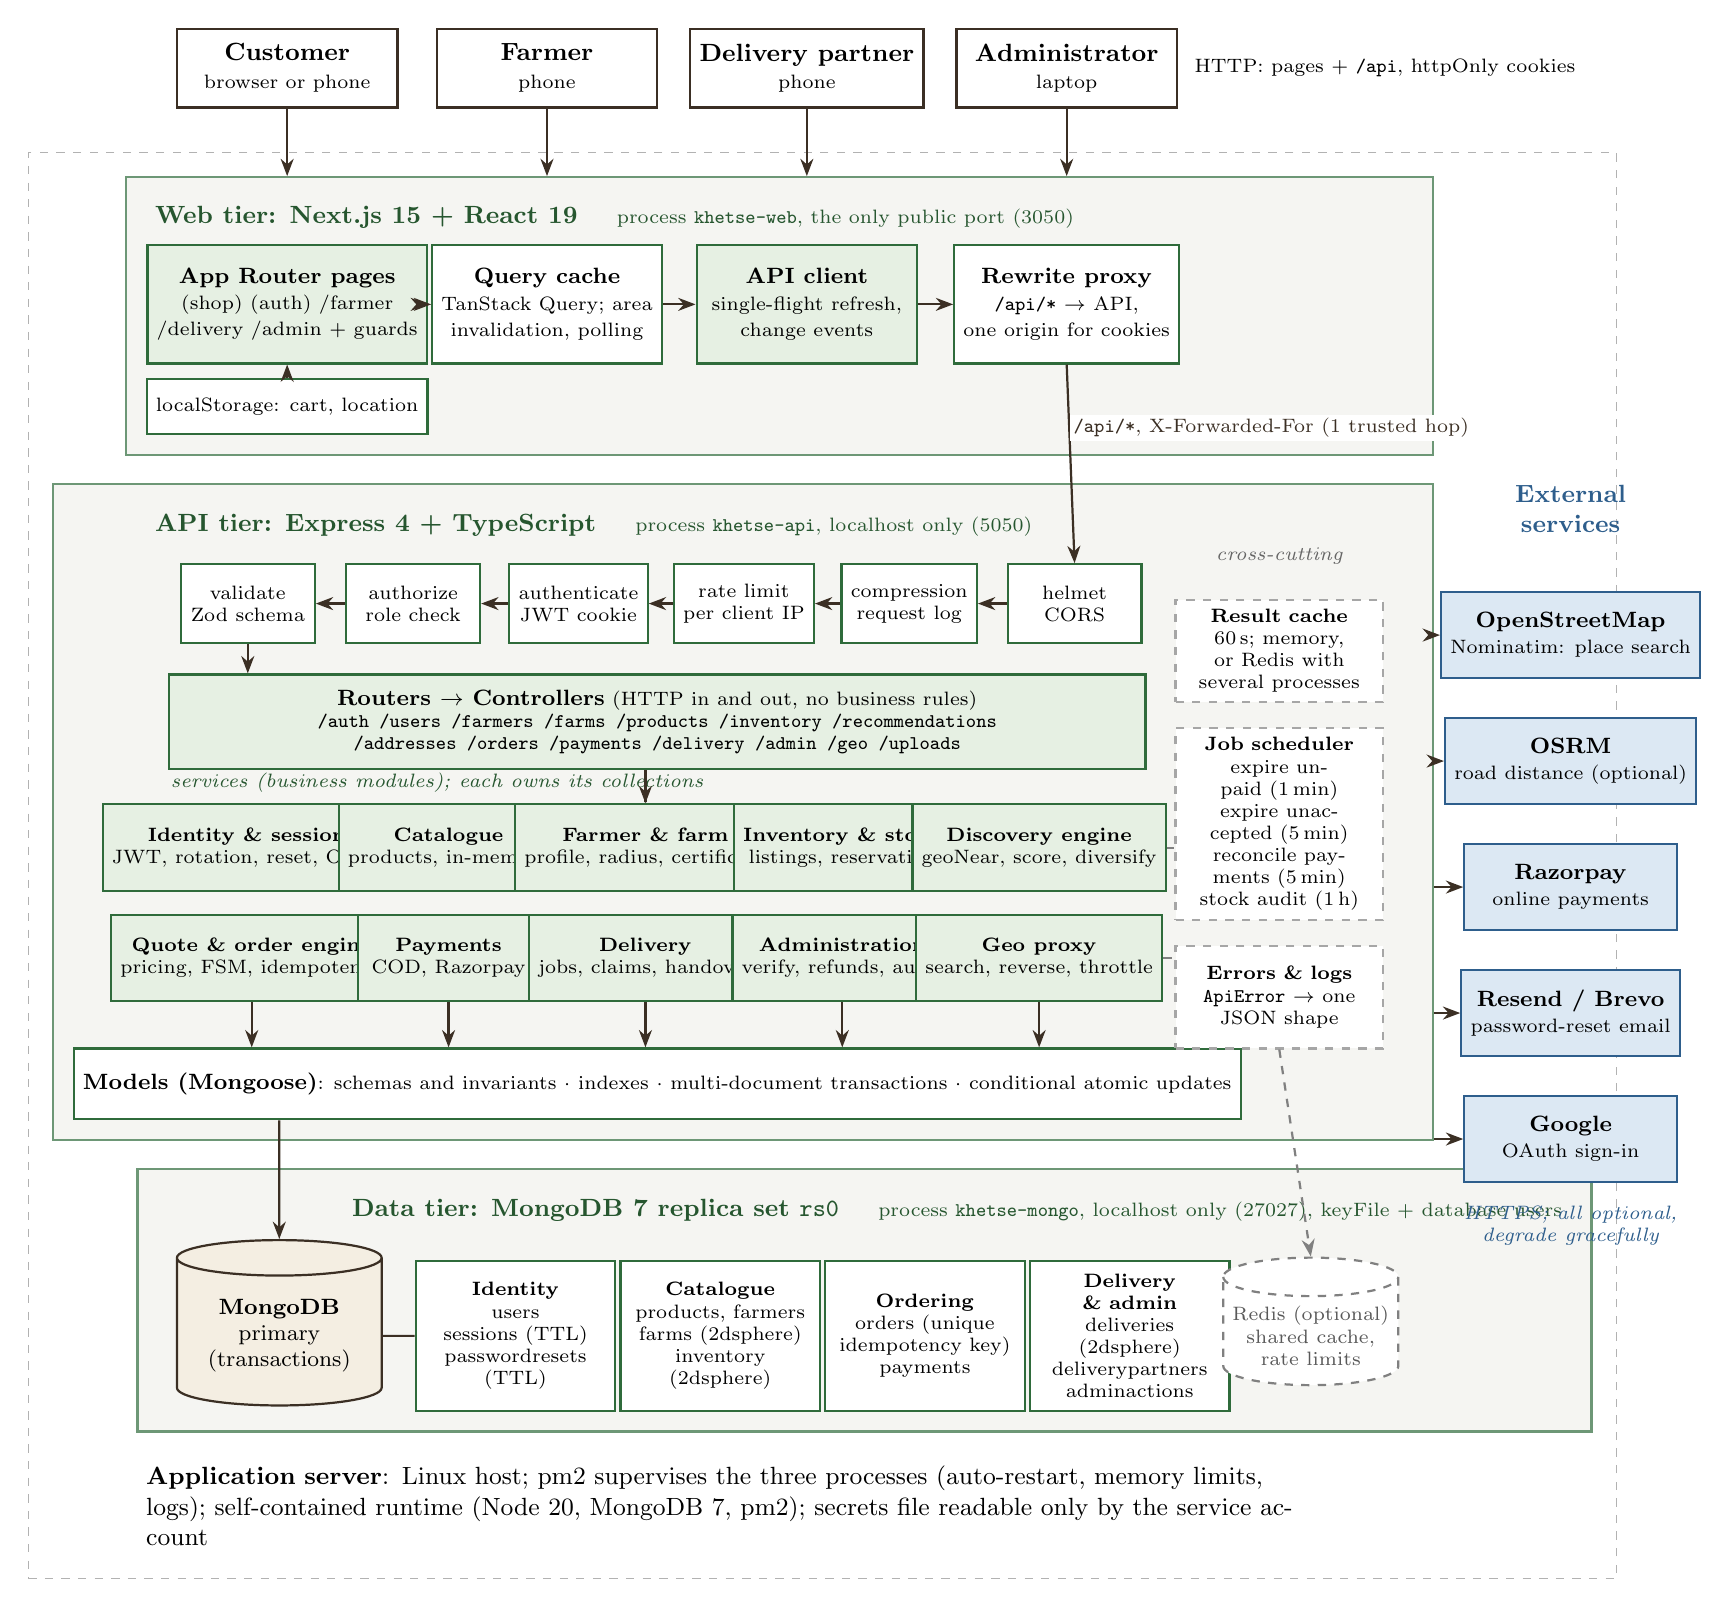
\begin{tikzpicture}[x=1mm, y=1mm, font=\footnotesize]
  % ---------------- Clients ----------------
  \foreach \x/\n/\t/\s in {17/cu/Customer/browser or phone, 50/fa/Farmer/phone, 83/pa/Delivery partner/phone, 116/ad/Administrator/laptop}
    \node[actor, minimum width=28mm, minimum height=10mm] (\n) at (\x,0) {\textbf{\t}\\[-1pt]\scriptsize \s};

  % ---------------- Web tier ----------------
  \node[tierlbl] (wl) at (-1,-19) {Web tier: Next.js 15 + React 19 \quad\normalfont\scriptsize process \texttt{khetse-web}, the only public port (3050)};
  \node[box, minimum width=28mm, minimum height=15mm, font=\footnotesize] (pages) at (17,-30) {\textbf{App Router pages}\\\scriptsize (shop) (auth) /farmer\\\scriptsize /delivery /admin + guards};
  \node[box, fill=white, minimum width=28mm, minimum height=15mm, font=\footnotesize] (qc) at (50,-30) {\textbf{Query cache}\\\scriptsize TanStack Query; area\\\scriptsize invalidation, polling};
  \node[box, minimum width=28mm, minimum height=15mm, font=\footnotesize] (ac) at (83,-30) {\textbf{API client}\\\scriptsize single-flight refresh,\\\scriptsize change events};
  \node[box, fill=white, minimum width=28mm, minimum height=15mm, font=\footnotesize] (px) at (116,-30) {\textbf{Rewrite proxy}\\\scriptsize \texttt{/api/*} $\to$ API,\\\scriptsize one origin for cookies};
  \draw[darr] (pages) -- (qc); \draw[arr] (qc) -- (ac); \draw[arr] (ac) -- (px);
  \node[sbox, fill=white, minimum width=28mm, font=\scriptsize] (ls) at (17,-43) {localStorage: cart, location};
  \draw[arr, dashed] (ls) -- (pages);
  \begin{scope}[on background layer]
    \coordinate (wr) at (160,-30);
    \node[tier, fit=(wl)(pages)(px)(ls)(wr)] (webz) {};
  \end{scope}
  \foreach \n in {cu,fa,pa,ad} \draw[arr] (\n.south) -- (\n.south |- webz.north);
  \node[font=\scriptsize, anchor=west] at (131,0) {HTTP: pages + \texttt{/api}, httpOnly cookies};

  % ---------------- API tier ----------------
  \node[tierlbl] (al) at (-1,-58) {API tier: Express 4 + TypeScript \quad\normalfont\scriptsize process \texttt{khetse-api}, localhost only (5050)};
  % middleware chain, right to left
  \foreach \x/\n/\t in {117/m1/{helmet\\CORS}, 96/m2/{compression\\request log}, 75/m3/{rate limit\\per client IP}, 54/m4/{authenticate\\JWT cookie}, 33/m5/{authorize\\role check}, 12/m6/{validate\\Zod schema}}
    \node[sbox, minimum width=17mm, minimum height=10mm, font=\scriptsize] (\n) at (\x,-68) {\t};
  \foreach \a/\b in {m1/m2,m2/m3,m3/m4,m4/m5,m5/m6} \draw[arr] (\a) -- (\b);
  \draw[arr] (px.south) -- node[lbl, right, pos=0.32]{\texttt{/api/*}, X-Forwarded-For (1 trusted hop)} (m1.north);

  \node[box, minimum width=124mm, minimum height=12mm, font=\scriptsize] (rt) at (64,-83) {\textbf{\footnotesize Routers $\to$ Controllers} (HTTP in and out, no business rules)\\ \texttt{/auth /users /farmers /farms /products /inventory /recommendations}\\ \texttt{/addresses /orders /payments /delivery /admin /geo /uploads}};
  \draw[arr] (m6.south) -- (m6.south |- rt.north);

  % services
  \foreach \x/\y/\n/\t/\s in {
      12.5/-99/s1/Identity \& sessions/{JWT, rotation, reset, OAuth},
      37.5/-99/s2/Catalogue/{products, in-memory},
      62.5/-99/s3/Farmer \& farm/{profile, radius, certificate},
      87.5/-99/s4/Inventory \& stock/{listings, reservation},
      112.5/-99/s5/Discovery engine/{geoNear, score, diversify},
      12.5/-113/s6/Quote \& order engine/{pricing, FSM, idempotency},
      37.5/-113/s7/Payments/{COD, Razorpay},
      62.5/-113/s8/Delivery/{jobs, claims, handover},
      87.5/-113/s9/Administration/{verify, refunds, audit},
      112.5/-113/s10/Geo proxy/{search, reverse, throttle}}
    \node[box, minimum width=23mm, minimum height=11mm, font=\scriptsize] (\n) at (\x,\y) {\textbf{\t}\\\s};
  \node[font=\scriptsize\itshape, anchor=south west, text=leaf!80!black] (svl) at (1,-93.2) {services (business modules); each owns its collections};
  \draw[arr] (rt.south -| s3) -- (svl.south -| s3) -- (s3.north);

  \node[box, fill=white, minimum width=124mm, minimum height=9mm, font=\scriptsize] (md) at (64,-129) {\textbf{\footnotesize Models (Mongoose)}: schemas and invariants $\cdot$ indexes $\cdot$ multi-document transactions $\cdot$ conditional atomic updates};
  \foreach \n in {s6,s7,s8,s9,s10} \draw[arr] (\n.south) -- (\n.south |- md.north);

  % cross-cutting column
  \node[font=\scriptsize\itshape, text=gray!80!black] (ccl) at (143,-62) {cross-cutting};
  \node[xbox, minimum width=25mm, minimum height=13mm, text width=24mm, font=\scriptsize] (cc1) at (143,-74) {\textbf{Result cache}\\60\,s; memory, or Redis with several processes};
  \node[xbox, minimum width=25mm, minimum height=22mm, text width=24mm, font=\scriptsize] (cc2) at (143,-96) {\textbf{Job scheduler}\\expire unpaid (1\,min)\\expire unaccepted (5\,min)\\reconcile payments (5\,min)\\stock audit (1\,h)};
  \node[xbox, minimum width=25mm, minimum height=13mm, text width=24mm, font=\scriptsize] (cc3) at (143,-118) {\textbf{Errors \& logs}\\\texttt{ApiError} $\to$ one JSON shape};
  \draw[gray, dashed, thick] (s5.east) -- (cc1.west |- s5.east);
  \draw[gray, dashed, thick] (s10.east) -- (cc2.west |- s10.east);

  \begin{scope}[on background layer]
    \coordinate (ar) at (160,-100);
    \node[tier, fit=(al)(m1)(m6)(rt)(md)(cc1)(cc3)(ccl)(ar)] (apiz) {};
  \end{scope}

  % ---------------- Data tier ----------------
  \node[tierlbl] (dl) at (24,-145) {Data tier: MongoDB 7 replica set \texttt{rs0} \quad\normalfont\scriptsize process \texttt{khetse-mongo}, localhost only (27027), keyFile + database users};
  \node[store, minimum width=26mm, minimum height=21mm, font=\footnotesize] (db) at (16,-161) {\textbf{MongoDB}\\primary\\(transactions)};
  \foreach \x/\n/\t in {
      46/c1/{\textbf{Identity}\\users\\sessions (TTL)\\passwordresets (TTL)},
      72/c2/{\textbf{Catalogue}\\products, farmers\\farms (2dsphere)\\inventory (2dsphere)},
      98/c3/{\textbf{Ordering}\\orders (unique\\idempotency key)\\payments},
      124/c4/{\textbf{Delivery \& admin}\\deliveries (2dsphere)\\deliverypartners\\adminactions}}
    \node[sbox, minimum width=24mm, minimum height=19mm, text width=23mm, font=\scriptsize] (\n) at (\x,-161) {\t};
  \draw[thick, soil] (db.east) -- (c1.west);
  \node[store, dashed, fill=white, draw=gray, text=gray!70!black, minimum width=22mm, minimum height=16mm, font=\scriptsize] (rd) at (147,-161) {Redis (optional)\\shared cache,\\rate limits};
  \draw[arr] (md.south -| db) -- (db.north);
  \draw[arr, gray, dashed] (cc3.south) -- (rd.north);
  \begin{scope}[on background layer]
    \coordinate (dr) at (160,-161); \coordinate (dlft) at (0.5,-161);
    \node[tier, fit=(dl)(db)(c4)(rd)(dr)(dlft)] (dbz) {};
  \end{scope}

  % ---------------- Server boundary ----------------
  \node[font=\small, anchor=north west, text width=150mm, align=left] (srv) at ($(dbz.south west)+(0,-3)$) {\textbf{Application server}: Linux host; pm2 supervises the three processes (auto-restart, memory limits, logs); self-contained runtime (Node 20, MongoDB 7, pm2); secrets file readable only by the service account};
  \begin{scope}[on background layer]
    \node[zone, fit=(webz)(apiz)(dbz)(srv)] (srvz) {};
  \end{scope}

  % ---------------- External services ----------------
  \node[font=\small\bfseries, text=skyd, align=center] (exl) at (180,-56) {External\\services};
  \foreach \y/\n/\t/\s in {-72/e1/OpenStreetMap/Nominatim: place search, -88/e2/OSRM/road distance (optional), -104/e3/Razorpay/online payments, -120/e4/{Resend / Brevo}/password-reset email, -136/e5/Google/OAuth sign-in}
    \node[ext, minimum width=27mm, minimum height=11mm, font=\footnotesize] (\n) at (180,\y) {\textbf{\t}\\\scriptsize \s};
  \foreach \n in {e1,e2,e3,e4,e5} \draw[arr] (apiz.east |- \n.west) -- (\n.west);
  \node[font=\scriptsize\itshape, text=skyd, align=center] at (180,-147) {HTTPS; all optional,\\degrade gracefully};
\end{tikzpicture}}}
\caption{Detailed high-level architecture. Users reach only the web tier, which serves the pages and proxies \texttt{/api} to the API on the same server. A request passes the middleware chain (right to left), a router and controller, one or more business services, and the model layer, which talks to the MongoDB replica set. Cross-cutting components (result cache, job scheduler, error handling) serve all modules. External services are called only by the API and are all optional.}
\label{fig:architecture}
\Description{Three stacked tiers inside one application server. Top: four user types (customer, farmer, delivery partner, administrator) send HTTP requests to the web tier. Web tier: App Router pages, a TanStack Query cache, an API client and a rewrite proxy, plus browser local storage for the cart and location. The proxy forwards /api requests to the API tier. API tier: a middleware chain of helmet and CORS, compression and request logging, per-IP rate limiting, JWT authentication, role authorization and Zod validation; then routers and controllers for fourteen route groups; then ten service modules (identity and sessions, catalogue, farmer and farm, inventory and stock, discovery engine, quote and order engine, payments, delivery, administration, geo proxy); then the Mongoose model layer. A cross-cutting column holds the result cache, the job scheduler with four jobs and error handling. Data tier: a MongoDB 7 replica set with collections grouped into identity, catalogue, ordering, and delivery and admin, and an optional Redis. On the right, external services: OpenStreetMap Nominatim, OSRM, Razorpay, Resend or Brevo, and Google OAuth.}
\end{figure}

\subsection{Components and their responsibilities}

\paragraph{Web tier.} The Next.js App Router renders pages grouped by audience: \texttt{(shop)} for customers and guests, \texttt{(auth)} for sign-in, and \texttt{/farmer}, \texttt{/delivery} and \texttt{/admin} for the three dashboards, which share one layout. A client-side guard redirects to login or explains which role a page needs; the API enforces the same rules independently. Data is read through one shared query cache (Section~\ref{sec:frontend}). The web server also \emph{rewrites} \texttt{/api/*} to the API, so the browser talks to a single origin.

\paragraph{API tier.} Every request passes the same middleware chain: security headers and CORS, compression, request logging, a per-client-IP rate limit, JWT authentication from an httpOnly cookie, a role check, and a Zod schema that validates and normalises the body, query and parameters. Routers map URLs to controllers, which only translate between HTTP and service calls. Services hold all business rules. Models declare schemas, invariants and indexes. Errors are raised as typed \texttt{ApiError}s and converted by one handler into a single response shape: \texttt{\{success, data, meta\}} or \texttt{\{success:false, error:\{code, message, details\}\}}.

\paragraph{Data tier.} A three-member-capable MongoDB replica set (one member at launch) provides 2dsphere indexes for geo queries, multi-document transactions for checkout, TTL indexes for expiring sessions and reset tokens, and atomic single-document updates for every contended write.

\paragraph{Communication.} Browser to web tier: HTTP with httpOnly session cookies. Web tier to API: HTTP over the loopback interface; the API trusts exactly one proxy hop to read the client's real IP for rate limiting. API to database: the MongoDB wire protocol with an authenticated application user. API to external services: HTTPS with timeouts; failures degrade a feature (for example, falling back to straight-line distance) instead of failing the request.

\begin{table}[htbp]
  \caption{Business modules and their boundaries. Each module's collections are written only by that module's services.}
  \label{tab:modules}
  \small
  \begin{tabularx}{\columnwidth}{@{}p{0.22\columnwidth}Lp{0.25\columnwidth}@{}}
    \toprule
    \textbf{Module} & \textbf{Responsibility} & \textbf{Owns} \\
    \midrule
    Identity \& sessions & Sign-up and login (mobile or email), token rotation, logout everywhere, password reset, Google OAuth & users, sessions, passwordresets \\
    Catalogue & Shared product definitions: name, type, shelf life, category; cached in memory & products \\
    Farmer \& farm & Profile, organic certificate, farm location, delivery radius & farmers, farms \\
    Inventory & Listings: price, unit, stock, dates, denormalised farm location & inventory \\
    Discovery & Geo retrieval, eligibility, scoring, diversity, radius widening, result cache & (reads only) \\
    Quote \& order engine & Server pricing, delivery fees, stock reservation, order state machine, idempotency & orders \\
    Payments & Cash-on-delivery records, Razorpay orders, signature checks, reconciliation & payments \\
    Delivery & Per-group delivery records, partner profiles, job board, claims, handover & deliveries, deliverypartners \\
    Administration & Overview, verification, suspension, admin cancellation, refunds, audit & adminactions \\
    Geo & Place search and reverse geocoding (proxied, cached, throttled) & (external) \\
    \bottomrule
  \end{tabularx}
\end{table}

\subsection{System context}

\begin{figure}[H]\centering
\fitbox{%
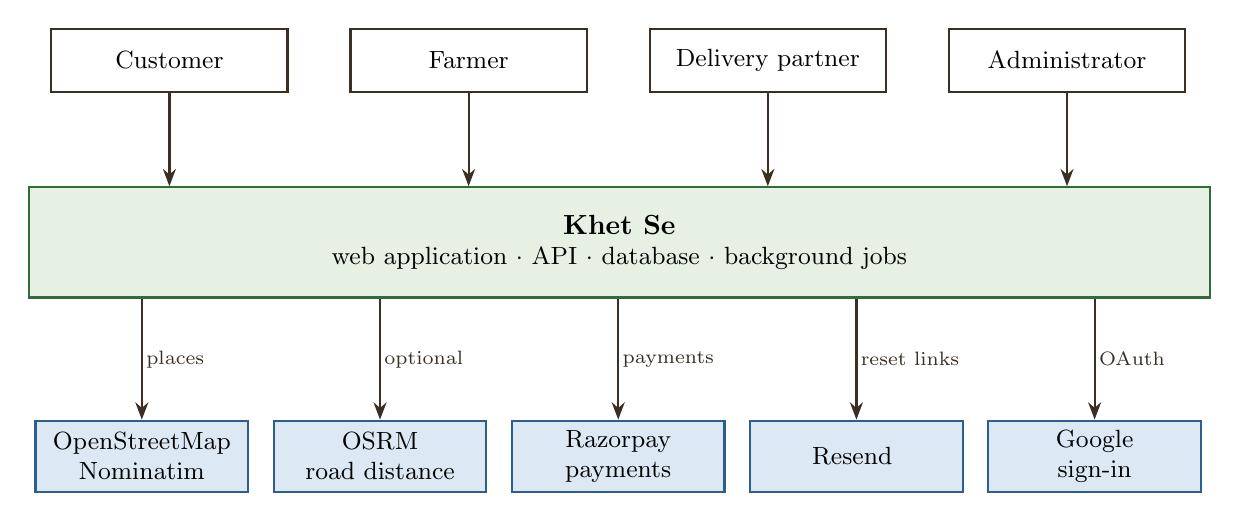
\begin{tikzpicture}
  \node[box, minimum width=150mm, minimum height=14mm, font=\normalsize] (sys) {\textbf{Khet Se}\\[-1pt]\small web application $\cdot$ API $\cdot$ database $\cdot$ background jobs};
  \foreach \i/\n/\t in {0/cust/Customer, 1/farm/Farmer, 2/part/Delivery partner, 3/adm/Administrator}
    \node[actor, minimum width=30mm] (\n) at ($(sys.north west)+(18mm+\i*38mm,16mm)$) {\t};
  \foreach \a in {cust,farm,part,adm} \draw[arr] (\a) -- (\a |- sys.north);
  \foreach \i/\n/\t in {0/osm/OpenStreetMap\\Nominatim, 1/osrm/OSRM\\road distance, 2/rzp/Razorpay\\payments, 3/mail/Resend / Brevo\\email, 4/goog/Google\\sign-in}
    \node[ext, minimum width=27mm] (\n) at ($(sys.south west)+(14.5mm+\i*30.25mm,-20mm)$) {\t};
  \foreach \e/\l in {osm/places, osrm/optional, rzp/payments, mail/reset links, goog/OAuth}
    \draw[arr] (sys.south -| \e) -- node[lbl,right]{\l} (\e);
\end{tikzpicture}}
\caption{System context: four kinds of users and the external services Khet Se depends on. Only the database is essential; every external service is optional or degrades gracefully.}
\label{fig:context}
\Description{A central Khet Se box with four user roles above it and five external services below it: OpenStreetMap Nominatim for places, OSRM for optional road distance, Razorpay for payments, Resend or Brevo for reset emails, and Google for OAuth sign-in.}
\end{figure}

\subsection{Deployment and delivery pipeline}

\begin{figure}[H]\centering
\fitbox{%
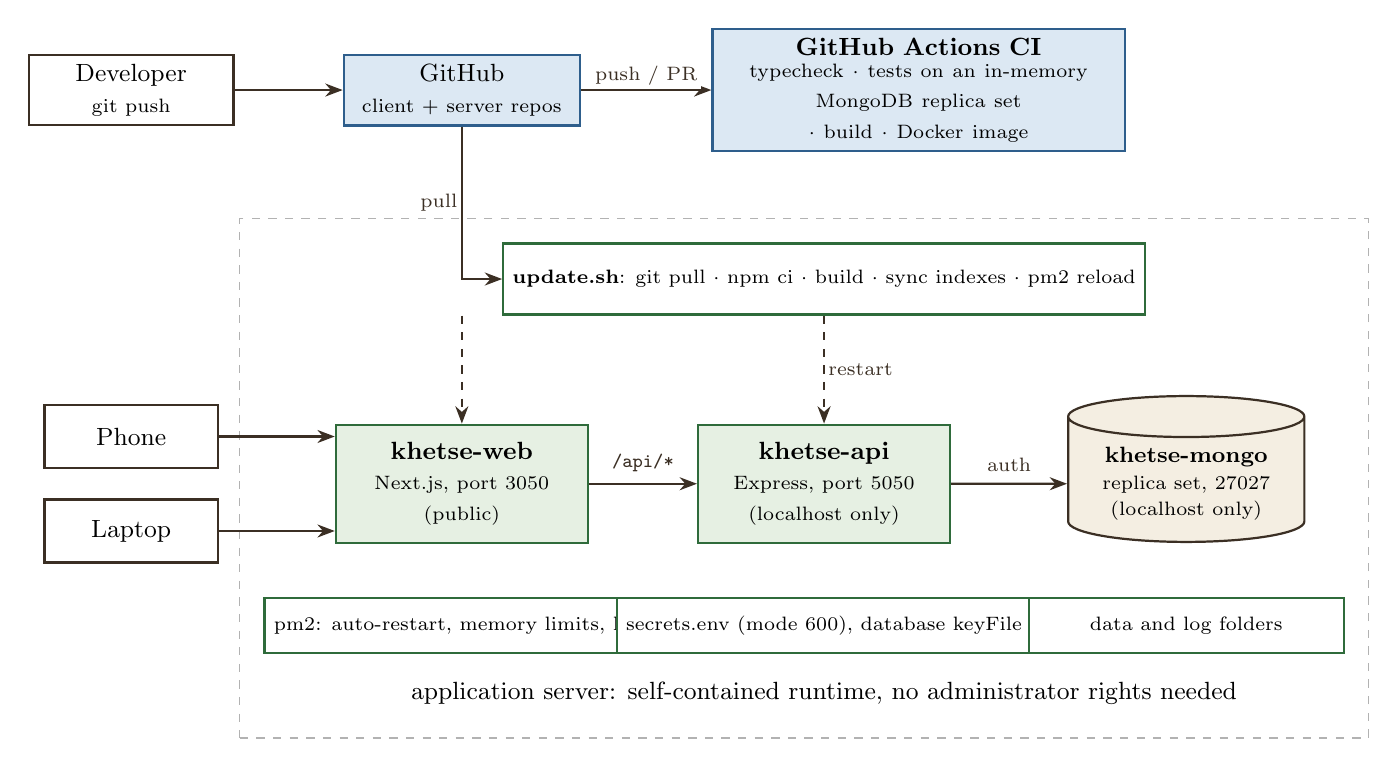
\begin{tikzpicture}[x=1mm, y=1mm, font=\footnotesize]
  \node[actor, minimum width=26mm] (dev) at (0,0) {Developer\\\scriptsize git push};
  \node[ext, minimum width=30mm] (gh) at (42,0) {GitHub\\\scriptsize client + server repos};
  \node[ext, minimum width=52mm, text width=50mm] (ci) at (100,0) {\textbf{GitHub Actions CI}\\\scriptsize typecheck $\cdot$ tests on an in-memory\\\scriptsize MongoDB replica set $\cdot$ build $\cdot$ Docker image};
  \draw[arr] (dev) -- (gh); \draw[arr] (gh) -- node[lbl,above]{push / PR} (ci);

  \node[box, fill=white, minimum width=70mm, font=\scriptsize] (up) at (88,-24) {\textbf{update.sh}: git pull $\cdot$ npm ci $\cdot$ build $\cdot$ sync indexes $\cdot$ pm2 reload};
  \draw[arr] (gh.south) |- node[lbl, pos=0.25, left]{pull} (up.west);

  \node[actor, minimum width=22mm] (b1) at (0,-44) {Phone};
  \node[actor, minimum width=22mm] (b2) at (0,-56) {Laptop};
  \node[box, minimum width=32mm, minimum height=15mm] (web) at (42,-50) {\textbf{khetse-web}\\\scriptsize Next.js, port 3050\\\scriptsize (public)};
  \node[box, minimum width=32mm, minimum height=15mm] (api) at (88,-50) {\textbf{khetse-api}\\\scriptsize Express, port 5050\\\scriptsize (localhost only)};
  \node[store, minimum width=30mm, minimum height=17mm, font=\footnotesize] (db) at (134,-50) {\textbf{khetse-mongo}\\\scriptsize replica set, 27027\\\scriptsize (localhost only)};
  \draw[arr] (b1.east) -- (b1.east -| web.west);
  \draw[arr] (b2.east) -- (b2.east -| web.west);
  \draw[arr] (web) -- node[lbl,above=1mm]{\texttt{/api/*}} (api);
  \draw[arr] (api) -- node[lbl,above=1mm]{auth} (db);
  \draw[arr, dashed] (up.south -| api) -- node[lbl, right]{restart} (api.north);
  \draw[arr, dashed] (up.south -| web) -- (web.north);

  \node[sbox, minimum width=40mm, font=\scriptsize] (k1) at (42,-68) {pm2: auto-restart, memory limits, logs};
  \node[sbox, minimum width=40mm, font=\scriptsize] (k2) at (88,-68) {secrets.env (mode 600), database keyFile};
  \node[sbox, minimum width=40mm, font=\scriptsize] (k3) at (134,-68) {data and log folders};
  \node[font=\small, anchor=north] (zl) at (88,-74) {application server: self-contained runtime, no administrator rights needed};
  \begin{scope}[on background layer]
    \node[zone, fit=(up)(web)(db)(api)(k1)(k3)(zl)] {};
  \end{scope}
\end{tikzpicture}}
\caption{Deployment and delivery. Every push is checked by CI. The server pulls, builds and restarts with one script. Only the web port is exposed; the API and database listen on localhost, and the database requires authentication.}
\label{fig:deploy}
\Description{A developer pushes to GitHub, which runs CI with typecheck, tests, build and Docker image. The application server pulls the code with update.sh and restarts the processes. Phones and laptops connect to khetse-web on the public port; it proxies /api to khetse-api on localhost, which talks to khetse-mongo on localhost. pm2, a secrets file and data folders support the processes.}
\end{figure}

\paragraph{Why proxy the API through the web server.} One origin removes cross-site cookie and CORS edge cases, exposes a single port, and lets the API trust exactly one proxy hop for the client's IP. \paragraph{Why pm2 and a self-contained runtime.} The service account on the target server has neither administrator rights nor Docker access. Node 20, MongoDB 7 and pm2 are therefore installed into one environment folder; pm2 supervises the three processes with automatic restart, memory limits and logs. Secrets (database passwords, JWT secret) are generated on the server into a file only the service account can read. The Dockerfiles, built in CI, keep a container deployment available where Docker is allowed.

\subsection{Back-end layers}

\begin{figure}[H]\centering
\fitbox{%
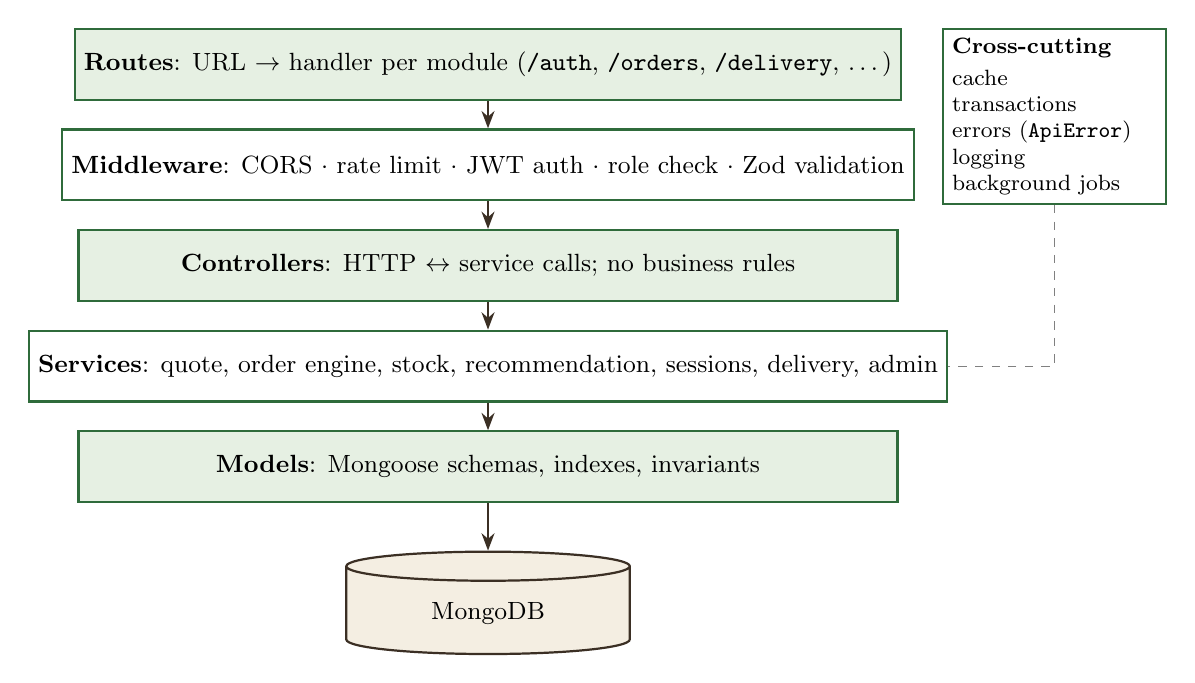
\begin{tikzpicture}[node distance=3.5mm, lay/.style={box, minimum width=104mm}]
  \node[lay] (r) {\textbf{Routes}: URL $\to$ handler per module (\texttt{/auth}, \texttt{/orders}, \texttt{/delivery}, \dots)};
  \node[lay, below=of r, fill=white] (m) {\textbf{Middleware}: CORS $\cdot$ rate limit $\cdot$ JWT auth $\cdot$ role check $\cdot$ Zod validation};
  \node[lay, below=of m] (c) {\textbf{Controllers}: HTTP $\leftrightarrow$ service calls; no business rules};
  \node[lay, below=of c, fill=white] (sv) {\textbf{Services}: quote, order engine, stock, recommendation, sessions, delivery, admin};
  \node[lay, below=of sv] (d) {\textbf{Models}: Mongoose schemas, indexes, invariants};
  \node[store, below=6mm of d, minimum width=36mm] (db) {MongoDB};
  \foreach \x/\y in {r/m,m/c,c/sv,sv/d,d/db} \draw[arr] (\x) -- (\y);
  \node[sbox, text width=26mm, minimum width=28mm, align=left, anchor=north west] (x) at ($(r.north east)+(5mm,0)$) {\textbf{Cross-cutting}\\[2pt] cache\\ transactions\\ errors (\texttt{ApiError})\\ logging\\ background jobs};
  \draw[gray, dashed] (x.south) -- (x.south |- sv.east) -- (sv.east);
\end{tikzpicture}}
\caption{Layers of the API. Each layer depends only on the one below, so services are tested without HTTP and can be reused by scripts and jobs.}
\label{fig:layers}
\Description{Five stacked layers: routes, middleware, controllers, services and models, above the MongoDB database, with a cross-cutting box for cache, transactions, errors, logging and background jobs.}
\end{figure}

\subsection{Key request flows}

\paragraph{Discovery.} Figure~\ref{fig:discovery} shows how ``what can I buy here?'' is answered with one indexed geo query and three batched reads; the algorithms are detailed in Section~\ref{sec:algorithms}.

\begin{figure}[H]\centering
\fitbox{%
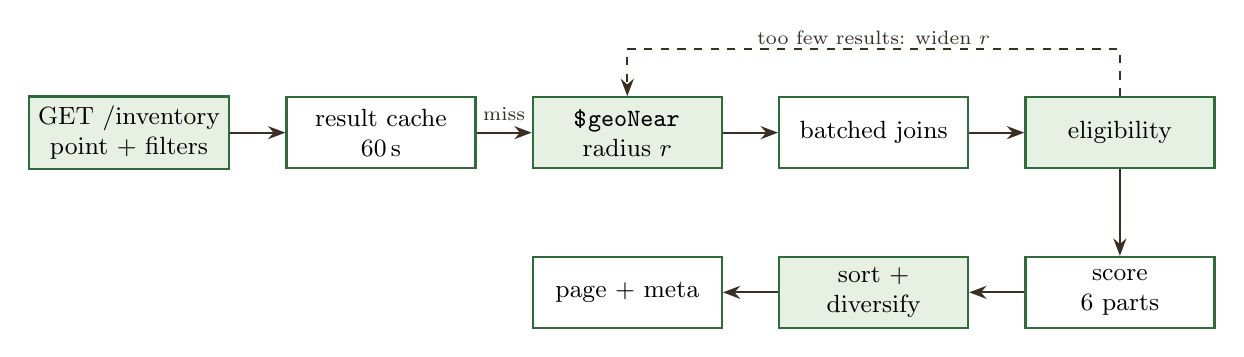
\begin{tikzpicture}[node distance=6mm and 7mm, every node/.style={font=\small}]
  \node[box, minimum width=24mm] (q) {GET /inventory\\point + filters};
  \node[box, right=of q, fill=white, minimum width=24mm] (c) {result cache\\60\,s};
  \node[box, right=of c, minimum width=24mm] (g) {\texttt{\$geoNear}\\radius $r$};
  \node[box, right=of g, fill=white, minimum width=24mm] (j) {batched joins};
  \node[box, right=of j, minimum width=24mm] (e) {eligibility};
  \node[box, below=11mm of e, fill=white, minimum width=24mm] (sc) {score\\6 parts};
  \node[box, left=of sc, minimum width=24mm] (dv) {sort +\\diversify};
  \node[box, left=of dv, fill=white, minimum width=24mm] (pg) {page + meta};
  \draw[arr] (q) -- (c); \draw[arr] (c) -- node[lbl,above=1mm]{miss} (g); \draw[arr] (g) -- (j); \draw[arr] (j) -- (e);
  \draw[arr] (e) -- (sc); \draw[arr] (sc) -- (dv); \draw[arr] (dv) -- (pg);
  \draw[arr, dashed] (e.north) -- ++(0,6mm) -| node[lbl,pos=0.25,above]{too few results: widen $r$} (g.north);
\end{tikzpicture}}
\caption{Discovery pipeline.}
\label{fig:discovery}
\Description{A request goes to a 60-second cache; on a miss, a geoNear query within radius r, batched joins and eligibility filtering run; if too few results, the radius is widened and the query repeats; then scoring, sorting with diversity, and pagination.}
\end{figure}

\paragraph{Checkout.} Figure~\ref{fig:checkout} shows placing an order: the cart is re-priced on the server, a repeated submission returns the original order, and the reservation of every line and the order insert commit together or not at all.

\begin{figure}[H]\centering
\fitbox{%
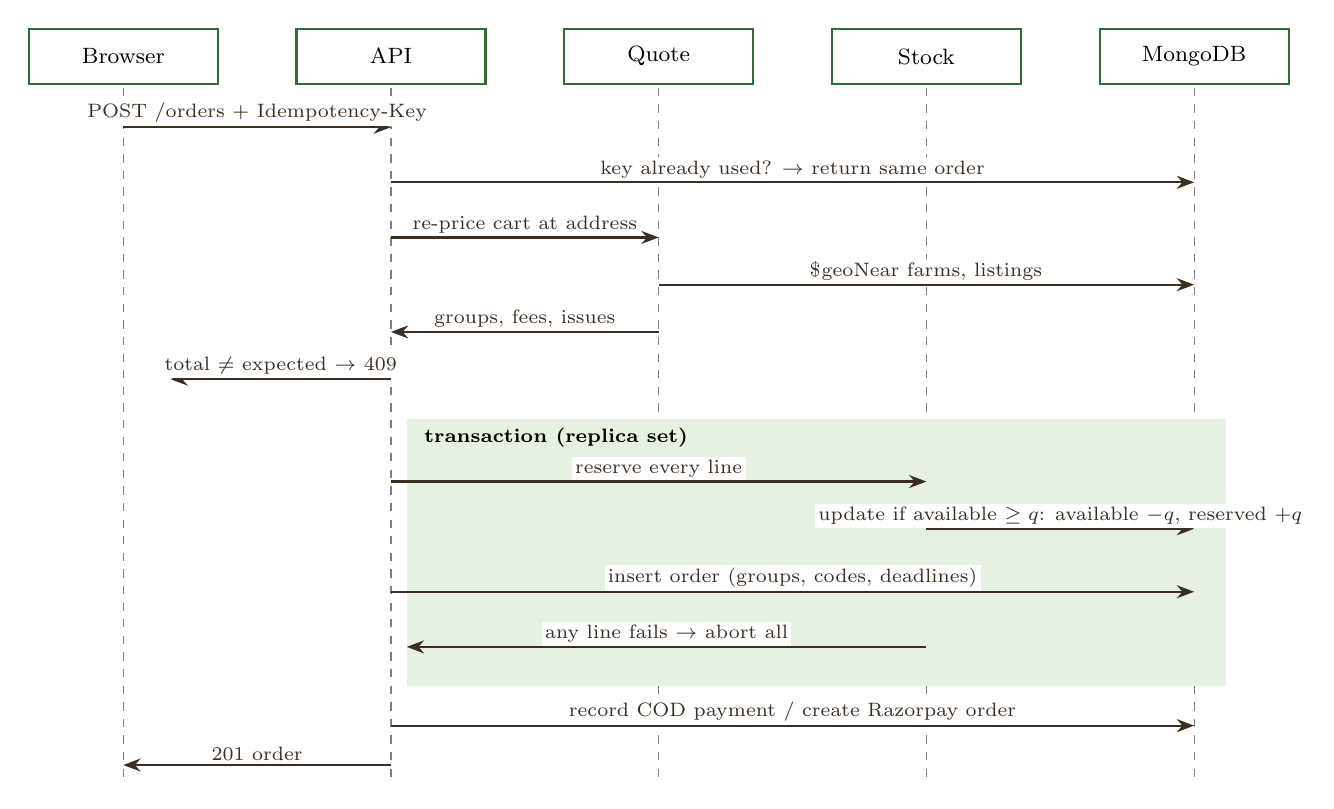
\begin{tikzpicture}[x=1mm, y=1mm, font=\footnotesize]
  \foreach \x/\n in {0/Browser, 34/API, 68/Quote, 102/Stock, 136/MongoDB}{
    \node[sbox, minimum width=24mm] (h\x) at (\x,0) {\n};
    \draw[gray, dashed] (\x,-4) -- (\x,-92);
  }
  \newcommand{\msg}[4]{\draw[arr] (#1,#3) -- node[lbl,above]{#4} (#2,#3);}
  \msg{0}{34}{-9}{POST /orders + Idempotency-Key}
  \msg{34}{136}{-16}{key already used? $\to$ return same order}
  \msg{34}{68}{-23}{re-price cart at address}
  \msg{68}{136}{-29}{\$geoNear farms, listings}
  \msg{68}{34}{-35}{groups, fees, issues}
  \draw[arr] (34,-41) -- node[lbl,above]{total $\ne$ expected $\to$ 409} (6,-41);
  \fill[leafl] (36,-46) rectangle (140,-80);
  \node[font=\scriptsize\bfseries, anchor=north west] at (37,-46) {transaction (replica set)};
  \msg{34}{102}{-54}{reserve every line}
  \msg{102}{136}{-60}{update if available $\ge q$: available $-q$, reserved $+q$}
  \msg{34}{136}{-68}{insert order (groups, codes, deadlines)}
  \draw[arr] (102,-75) -- node[lbl,above]{any line fails $\to$ abort all} (36,-75);
  \msg{34}{136}{-85}{record COD payment / create Razorpay order}
  \draw[arr] (34,-90) -- node[lbl,above]{201 order} (0,-90);
\end{tikzpicture}}
\caption{Placing an order: idempotency, server re-pricing and an all-or-nothing stock reservation.}
\label{fig:checkout}
\Description{Sequence diagram between browser, API, quote service, stock service and MongoDB. The idempotency key is checked, the cart is re-priced with geoNear, a price mismatch returns 409, then inside a transaction each line is reserved with a conditional update and the order is inserted; any failure aborts all; finally the payment is recorded and 201 is returned.}
\end{figure}

\paragraph{Delivery by a partner.} Figure~\ref{fig:delivery}: two partners may accept the same job at the same moment; one conditional update decides the winner, and only the winner receives addresses and phone numbers.

\begin{figure}[H]\centering
\fitbox{%
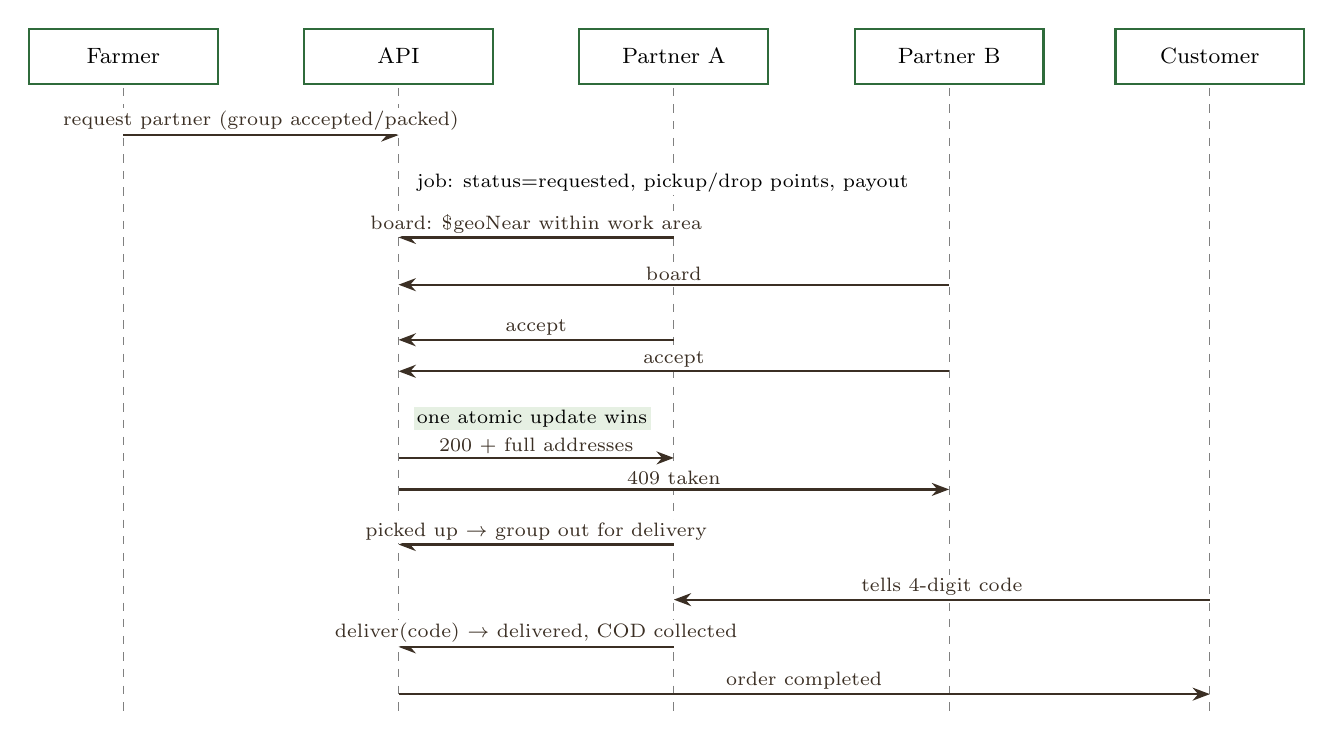
\begin{tikzpicture}[x=0.92mm, y=1mm, font=\footnotesize]
  \foreach \x/\n in {0/Farmer, 38/API, 76/Partner A, 114/Partner B, 150/Customer}{
    \node[sbox, minimum width=24mm] at (\x,0) {\n};
    \draw[gray, dashed] (\x,-4) -- (\x,-84);
  }
  \newcommand{\msg}[4]{\draw[arr] (#1,#3) -- node[lbl,above]{#4} (#2,#3);}
  \msg{0}{38}{-10}{request partner (group accepted/packed)}
  \node[lbl, anchor=west] at (40,-16) {job: status=requested, pickup/drop points, payout};
  \msg{76}{38}{-23}{board: \$geoNear within work area}
  \msg{114}{38}{-29}{board}
  \msg{76}{38}{-36}{accept}
  \msg{114}{38}{-40}{accept}
  \node[lbl, anchor=west, fill=leafl] at (40,-46) {one atomic update wins};
  \msg{38}{76}{-51}{200 + full addresses}
  \msg{38}{114}{-55}{409 taken}
  \msg{76}{38}{-62}{picked up $\to$ group out for delivery}
  \msg{150}{76}{-69}{tells 4-digit code}
  \msg{76}{38}{-75}{deliver(code) $\to$ delivered, COD collected}
  \msg{38}{150}{-81}{order completed}
\end{tikzpicture}}
\caption{Delivery job life cycle with a first-wins claim.}
\label{fig:delivery}
\Description{Sequence diagram: the farmer requests a partner; two partners load the job board and both accept; one atomic update wins, the winner gets addresses and the other gets 409; the winner picks up, receives the code from the customer and completes delivery.}
\end{figure}

\paragraph{Authentication.} Figure~\ref{fig:auth}: short-lived access tokens are renewed with a refresh token that changes on every use; replaying an old token revokes the whole session family.

\begin{figure}[H]\centering
\fitbox{%
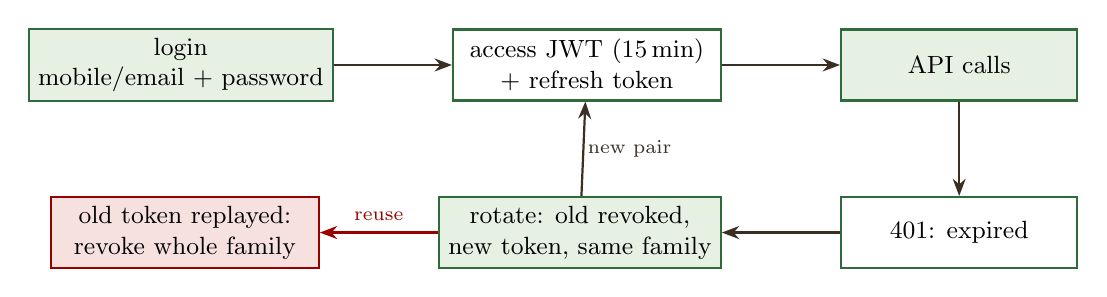
\begin{tikzpicture}[node distance=8mm and 15mm]
  \node[box, minimum width=34mm] (login) {login\\mobile/email + password};
  \node[box, right=of login, fill=white, minimum width=34mm] (pair) {access JWT (15\,min)\\+ refresh token};
  \node[box, right=of pair, minimum width=30mm] (use) {API calls};
  \node[box, below=12mm of use, fill=white, minimum width=30mm] (exp) {401: expired};
  \node[box, left=of exp, minimum width=34mm] (rot) {rotate: old revoked,\\new token, same family};
  \node[bad, left=of rot, minimum width=34mm] (reuse) {old token replayed:\\revoke whole family};
  \draw[arr] (login) -- (pair); \draw[arr] (pair) -- (use); \draw[arr] (use) -- (exp);
  \draw[arr] (exp) -- (rot);
  \draw[arr] (rot) -- node[lbl,right]{new pair} (pair);
  \draw[arr, red!60!black] (rot) -- node[lbl,above=1mm]{reuse} (reuse);
\end{tikzpicture}}
\caption{Session renewal with refresh-token rotation and reuse detection.}
\label{fig:auth}
\Description{Login issues an access token and a refresh token; API calls continue until a 401; the refresh token is rotated within the same family; replaying an old token revokes the whole family.}
\end{figure}

\subsection{Order state machine}

\begin{figure}[H]\centering
\fitbox{%
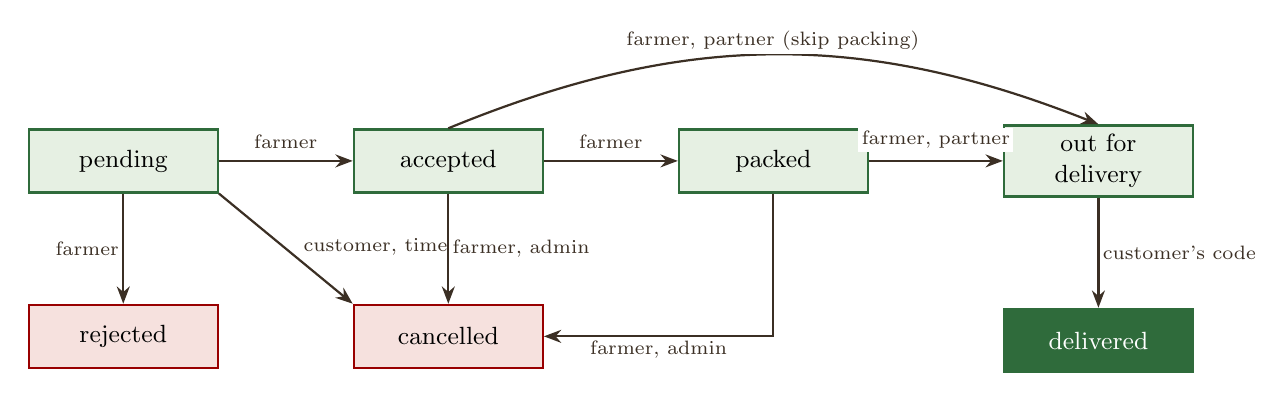
\begin{tikzpicture}[node distance=12mm and 17mm]
  \node[state] (p) {pending};
  \node[state, right=of p] (a) {accepted};
  \node[state, right=of a] (k) {packed};
  \node[state, right=of k] (o) {out for\\delivery};
  \node[state, below=14mm of o, fill=leaf, text=white] (d) {delivered};
  \node[bad, below=14mm of p] (r) {rejected};
  \node[bad, below=14mm of a] (c) {cancelled};
  \draw[arr] (p) -- node[lbl,above=1mm]{farmer} (a);
  \draw[arr] (a) -- node[lbl,above=1mm]{farmer} (k);
  \draw[arr] (k) -- node[lbl,above=1mm]{farmer, partner} (o);
  \draw[arr] (a.north) to[bend left=22] node[lbl,above]{farmer, partner (skip packing)} (o.north);
  \draw[arr] (o) -- node[lbl,right]{customer's code} (d);
  \draw[arr] (p) -- node[lbl,left]{farmer} (r);
  \draw[arr] (p.south east) -- node[lbl,pos=0.6,above right]{customer, timeout} (c.north west);
  \draw[arr] (a) -- node[lbl,right]{farmer, admin} (c);
  \draw[arr] (k.south) |- node[lbl,pos=0.75,below]{farmer, admin} (c.east);
\end{tikzpicture}}
\caption{Life cycle of one farm's part (group) of an order. Each transition is one conditional update that applies only if the current status is an allowed source.}
\label{fig:fsm}
\Description{States pending, accepted, packed, out for delivery and delivered, with rejected and cancelled as failure states, and the actor allowed to make each transition.}
\end{figure}

The order's own status (\emph{placed, in progress, completed, cancelled}) and its payment status are \emph{derived} from its groups after every transition, never edited directly. Stock is released when a group is rejected or cancelled and consumed when it is delivered. When a partner delivers, farmers can no longer mark the group out for delivery or delivered, so two actors can never both complete it.

\subsection{Consistency and concurrency}

\begin{itemize}
  \item \textbf{Conditional updates as the unit of correctness.} Every contended write is one document update with its precondition in the filter: stock (\texttt{available $\ge q$}), transitions (\texttt{status $\in$ allowed}), job claims (\texttt{status = requested, partner = null}) and refund records (document version). The database serialises them; no application locks exist.
  \item \textbf{Transactions where several documents change together.} Reserving every line and inserting the order happen in one multi-document transaction. On a standalone development database, the same code falls back to compensation (releasing reservations already made).
  \item \textbf{Idempotency.} A unique \texttt{(customer, idempotencyKey)} index makes retries and double taps return the original order.
  \item \textbf{Safety nets.} An hourly job recomputes reserved stock from open orders and reports drift; a reconciliation job asks Razorpay about payments whose callback never arrived before an unpaid order is cancelled.
\end{itemize}

\subsection{Security architecture}

\begin{table}[htbp]
  \caption{Threats and controls}
  \label{tab:security}
  \small
  \begin{tabularx}{\columnwidth}{@{}p{0.22\columnwidth}L@{}}
    \toprule
    \textbf{Threat} & \textbf{Control} \\
    \midrule
    Stolen session & 15-minute access tokens; refresh tokens stored only as SHA-256 hashes, rotated on every use, revoked as a family on reuse; httpOnly cookies; logout everywhere; suspension ends all sessions. \\
    Password guessing & bcrypt hashes; 20 attempts per 15 minutes per IP on credential endpoints; identical errors for unknown account and wrong password. \\
    Account enumeration & Password reset answers identically for unknown accounts and sends mail in the background, so timing reveals nothing. \\
    Fake delivery & 4-digit code known only to the customer; wrong attempts counted atomically, locked after 5 ($\le 0.05\%$ success by guessing). \\
    Privilege abuse & Role checks on every route; partners see contacts only for jobs they hold; farmers never see handover codes; admin actions audited with a mandatory reason for negative decisions. \\
    Bad input & Zod validation of every input; regular expressions only from escaped text; images only from approved hosts. \\
    Network exposure & API and database on localhost only; database authentication with separate admin and application users; one public port. \\
    \bottomrule
  \end{tabularx}
\end{table}

\subsection{Caching strategy}

\begin{table}[htbp]
  \caption{Caching layers and how each stays correct}
  \label{tab:caching}
  \small
  \begin{tabularx}{\columnwidth}{@{}p{0.2\columnwidth}p{0.22\columnwidth}L@{}}
    \toprule
    \textbf{Layer} & \textbf{What} & \textbf{Freshness rule} \\
    \midrule
    Browser (HTTP) & public lists & \texttt{no-cache} + ETag: always revalidated; \texttt{304} when unchanged. \\
    Client query cache & each screen's data & 15\,s fresh; refetch on focus; invalidated by area after writes; polling for live queues. \\
    API result cache & discovery results & 60\,s; key rounds coordinates to $\approx$110\,m; cleared on any farm, listing, stock or verification change; memory or Redis. \\
    Catalogue cache & product definitions & short TTL; the catalogue rarely changes. \\
    Geocoding & place search & cached and throttled to respect OpenStreetMap's usage policy. \\
    \bottomrule
  \end{tabularx}
\end{table}

\subsection{Scaling path}

\begin{enumerate}
  \item \textbf{Several API processes} (one per core) behind the web proxy or a load balancer, with Redis for the shared result cache and rate limits. The API is stateless, so this needs no code change.
  \item \textbf{Native bcrypt} on the thread pool, so bursts of logins do not block other requests (Section~\ref{sec:performance}).
  \item \textbf{A job queue} so scheduled work runs once across many processes.
  \item \textbf{Push instead of polling} (server-sent events) for job boards and order queues, the largest share of steady traffic.
  \item \textbf{Shard by city.} Farms, listings and orders are local to a city, so cities partition naturally.
\end{enumerate}

\subsection{Technology Stack}

\begin{table}[htbp]
  \caption{Technology stack, reasons and alternatives considered}
  \label{tab:stack}
  \small
  \begin{tabularx}{\columnwidth}{@{}p{0.17\columnwidth}p{0.25\columnwidth}L@{}}
    \toprule
    \textbf{Layer} & \textbf{Technology} & \textbf{Reason (alternatives)} \\
    \midrule
    Language & TypeScript (Node.js 20) & One typed language on both sides; shared validation style. (Java/Spring, Python/Django: heavier for a small team.) \\
    Web framework & Next.js 15, React 19 & File-based routing, route groups per audience, built-in rewrites for the same-origin proxy. (Plain React SPA: no server proxy or routing conventions.) \\
    UI & Tailwind CSS, Radix primitives, Lucide icons, Leaflet maps & Small, accessible components; OpenStreetMap tiles without licence cost. (Google Maps: billing.) \\
    Client state & TanStack Query 5, React Hook Form + Zod & Shared cache with invalidation and polling; typed forms. (Redux: more boilerplate for server state.) \\
    API & Express 4, Zod, helmet, express-rate-limit, compression & Mature, minimal, easy to layer. (NestJS: more structure than needed.) \\
    Database & MongoDB 7 (replica set), Mongoose 8 & Native 2dsphere indexes and \texttt{\$geoNear}, transactions, flexible order documents. (PostgreSQL + PostGIS: equally capable; MongoDB chosen for embedded order groups.) \\
    Auth & jsonwebtoken, bcryptjs, Google OAuth with PKCE & Stateless access tokens plus server-side refresh sessions. \\
    External & Razorpay, Resend/Brevo, Nominatim, OSRM & Indian payments; HTTP email APIs (avoiding a vulnerable SMTP library); free geocoding. \\
    Testing & Vitest, Supertest, mongodb-memory-server & Real HTTP against a real in-memory replica set, so transactions are tested. \\
    Operations & pm2, GitHub Actions, Docker & Supervision without root; CI on every push; images for container hosts. \\
    \bottomrule
  \end{tabularx}
\end{table}

%% =====================================================================
\section{Methodology}
\label{sec:methodology}

The system was built iteratively, one capability at a time, each followed by tests: first identity, catalogue and farms; then discovery and ranking; then ordering and payments; then the delivery-partner role; then administration. Each phase began with the requirement and its failure modes (for example, ``two buyers race for the last kilogram''), chose the simplest mechanism that provably prevents the failure, and added an integration test that reproduces the race. Algorithms were chosen for explainability and correctness at city scale rather than theoretical optimality; parameters are configuration, not code. After the features were complete, an independent checker and a workload model were built to validate the algorithms and the capacity assumptions against the running system. \aiuse

\subsection{Data Collection and Preparation}

\begin{itemize}
  \item \textbf{Catalogue.} A curated list of common vegetables, fruits, grains, pulses and dry goods with English, Hindi and local names, category, and type: \emph{fresh} items carry a shelf life in days; \emph{dry} items carry processing and expiry dates.
  \item \textbf{Locations.} Coordinates for 22 Durg--Bhilai localities and 10 surrounding villages were obtained from OpenStreetMap (Nominatim, through the application's own geo endpoint) and stored in a JSON file. This replaced hand-placed demo coordinates, some of which were found to be 5--7\,km wrong.
  \item \textbf{Demo data.} Seed scripts create farms, farmers, listings, customers, delivery partners, an administrator and realistic order histories for Raipur and Durg--Bhilai, so every screen shows a platform in use.
  \item \textbf{Algorithm test bed.} 21 farms (59 listings) and 27 customers at real places, each farm designed to exercise one rule (Section~\ref{sec:validation}).
  \item \textbf{Input normalisation.} Every input is parsed by a Zod schema that trims, coerces and defaults it; the parsed value replaces the raw input. Mobile numbers written as \texttt{+91 98111 00099}, \texttt{098111 00099} or \texttt{9811100099} all become ten digits; coordinates are validated as longitude and latitude ranges; missing optional fields (email, certificate) are stored as absent, never as empty strings, so partial unique indexes work.
  \item \textbf{Limitations.} Ratings and order histories in the demo data are synthetic; real behaviour will differ. Straight-line distance is used when road distance is unavailable.
\end{itemize}

\subsection{Analysis / Processing Method}
\label{sec:algorithms}

\begin{table}[htbp]
  \caption{Algorithms used ($n$ indexed documents, $k$ candidates near the customer, $m$ page size)}
  \label{tab:algos}
  \small
  \begin{tabularx}{\columnwidth}{@{}p{0.27\columnwidth}p{0.22\columnwidth}p{0.11\columnwidth}L@{}}
    \toprule
    \textbf{Algorithm} & \textbf{Used in} & \textbf{Cost} & \textbf{Why here} \\
    \midrule
    2dsphere index + \texttt{\$geoNear} & discovery, job board, checkout & $O(\log n + k)$ & exact spherical distances, sorted, index-backed \\
    Adaptive radius widening & discovery & $\le 3$ queries & local in dense areas, results in sparse ones \\
    Hybrid weighted scoring & product and farm ranking & $O(k)$ & transparent, tunable, no history needed \\
    Bayesian average rating & ranking & $O(1)$ & one 5-star review must not beat 200 good ones \\
    Grouped min--max price & ranking & $O(k)$ & compares only like-for-like offers \\
    Greedy diversity re-rank & recommended order & $O(k\,m)$ & one farm cannot fill the first page \\
    Conditional atomic update & stock, transitions, claims & $O(1)$ & correctness without locks \\
    Finite-state machine & order groups & $O(1)$ & illegal transitions impossible \\
    Token rotation, reuse detection & sessions & $O(1)$ & detects stolen refresh tokens \\
    Attempt-counted code & handover & $O(1)$ & guessing bounded at 0.05\% \\
    \bottomrule
  \end{tabularx}
\end{table}

\paragraph{Geo-spatial retrieval.} For a customer at $P$, every listing whose farm lies within the search radius $r$ \emph{and} delivers to $P$ (its own radius $R_f$) must be found in distance order. Points are GeoJSON with a 2dsphere index; \texttt{\$geoNear} walks the index outward from $P$ and returns candidates sorted by great-circle distance
\[
  d(P,Q) = 2R\arcsin\sqrt{\sin^2\tfrac{\Delta\varphi}{2} + \cos\varphi_P\cos\varphi_Q\sin^2\tfrac{\Delta\lambda}{2}}.
\]
Listing-level eligibility is applied inside the index scan; the per-farm condition $d(P,f) \le R_f$ is applied after joining farms. Instead of a lookup per candidate, the distinct farm, farmer and product ids are loaded with one \texttt{\$in} query each, which on a city-sized benchmark replaced about 3{,}000 per-document lookups per request with three reads. \emph{Alternatives:} haversine in application code is $O(n)$ per request; geohash or H3 grids need neighbour expansion and still need exact distances; a separate search engine adds an operational component for a capability the database already has.

\begin{algorithm}[H]
\caption{Adaptive radius selection}
\label{alg:radius}
\begin{pseudo}
  \item \kw{input:} point $P$; steps $S = [8, 15, 25]$\,km; minimum results $N$ (8 products or 4 farms)
  \item \kw{for} $r \in S$ \kw{do}
  \item \ind $C \gets$ eligible candidates within $r$
  \item \ind \kw{if} $|C| \ge N$ \kw{then return} $(C, r)$
  \item \kw{return} $(C, \text{last } r)$ \hfill \emph{the response says the search was widened}
\end{pseudo}
\end{algorithm}

\noindent In a dense neighbourhood the closest farms are shown, not cheaper farms 20\,km away; on the city's edge, results still appear and the interface says that farms further away are included. A radius chosen by the user is respected exactly.

\paragraph{Hybrid weighted scoring.} Each candidate gets six component scores $s_i \in [0,1]$ combined as $\text{score} = \sum_i w_i s_i / \sum_i w_i$ with weights proximity $0.30$, freshness $0.20$, stock $0.10$, rating $0.15$, price $0.15$ and organic $0.10$.

\begin{table}[htbp]
  \caption{Score components}
  \label{tab:score}
  \small
  \begin{tabularx}{\columnwidth}{@{}p{0.15\columnwidth}p{0.4\columnwidth}L@{}}
    \toprule
    \textbf{Part} & \textbf{Formula} & \textbf{Reasoning} \\
    \midrule
    Proximity & $1 - d/r$ & closer is fresher and cheaper to deliver \\
    Freshness & fresh: $1 - \text{age}/\text{shelfLife}$; dry: $\frac{\text{expiry}-\text{now}}{\text{expiry}-\text{processed}}$ & remaining usable life \\
    Stock & $\min\!\big(1, \frac{\text{available}}{10\cdot\text{minOrder}}\big)$ & can serve many orders; saturates \\
    Rating & $\big(\frac{\bar r\,n + 3.5\cdot 5}{n + 5} - 1\big)/4$ & Bayesian average toward prior 3.5 \\
    Price & $\frac{p_{\max} - p}{p_{\max} - p_{\min}}$ within (product, unit, pack) & like-for-like only \\
    Organic & 1 if the certificate is verified & claims alone do not count \\
    \bottomrule
  \end{tabularx}
\end{table}

\noindent \emph{Why not machine learning:} at launch there is no interaction history (cold start). A weighted model works from the first day, can be explained to farmers (``your tomatoes are 5 days old''), and is tuned by configuration. Every part is returned with each result, so the ranking is auditable; later, the same parts become features for a learning-to-rank model. \emph{Bayesian rating example:} one 5-star review gives $(5 + 17.5)/6 = 3.75$; 200 reviews averaging 4.7 give $(940 + 17.5)/205 \approx 4.67$, so the established farmer ranks higher.

\begin{algorithm}[H]
\caption{Farm-diversity re-rank (decay $\delta = 0.85$)}
\label{alg:diversity}
\begin{pseudo}
  \item \kw{input:} items sorted by score; page size $m$
  \item $\text{picked}[f] \gets 0$ for every farm $f$; $\text{out} \gets [\,]$
  \item \kw{while} $|\text{out}| < m$ \kw{and} items remain \kw{do}
  \item \ind choose the item $x$ maximising $\text{score}(x)\cdot\delta^{\,\text{picked}[\text{farm}(x)]}$
  \item \ind append $x$ to out; $\text{picked}[\text{farm}(x)] \gets \text{picked}[\text{farm}(x)] + 1$
  \item \kw{return} out followed by the remaining items in score order
\end{pseudo}
\end{algorithm}

\noindent In the spirit of maximal marginal relevance, the soft penalty lets customers compare farms and gives small farms visibility, while an outstanding second item from the same farm still appears early. Cost is $O(k\,m)$ for the page only. Explicit sorts (distance, price, freshness) keep their exact order.

\paragraph{Sellability rule.} One predicate, shared by search, farm lists, product pages, farmer profiles and checkout, decides whether a listing can be sold now:
\[
\text{sellable} \iff \text{active} \wedge \text{available} \ge \text{minOrder} \wedge
\begin{cases}
\text{now} - \text{harvest} \le \text{shelfLife} & \text{fresh}\\
\text{expiry} > \text{now} & \text{dry}
\end{cases}
\]
It is compiled once into a database filter so the geo query applies it inside the index scan, making ``shown'' and ``orderable'' the same set by construction.

\begin{algorithm}[H]
\caption{Reserve stock for an order (inside one transaction)}
\label{alg:reserve}
\begin{pseudo}
  \item \kw{for each} line $(\ell, q)$ \kw{do}
  \item \ind \texttt{updateOne(\{\_id: $\ell$, available: \{\$gte: $q$\}\}, \{\$inc: \{available: $-q$, reserved: $+q$\}\})}
  \item \ind \kw{if} no document matched \kw{then} abort the transaction; report ``only $x$ left''
  \item insert the order; commit
\end{pseudo}
\end{algorithm}

\noindent The check and the decrement are one atomic operation, so two buyers racing for the last units cannot both succeed. Locks would serialise all checkouts; read-then-write would oversell.

\paragraph{Delivery job matching.} A partner's board is a \texttt{\$geoNear} from the partner's base within their work area, filtered to \texttt{status = requested}, nearest pickup first. Claiming is \texttt{findOneAndUpdate(\{\_id, status: requested, partner: null\}, \{status: assigned, partner: me\})}; payout is $\max(30,\, 20 + 6\cdot\text{tripKm})$ rupees, and a partner may hold at most 3 jobs. Centrally optimal assignment (Hungarian algorithm, vehicle routing) pays off with large full-time fleets; at launch, partners are part-time, know local roads and each job is one pickup and one drop, so a geo-filtered board with an atomic claim is simpler, fairer and correct under concurrency.

\paragraph{Session security.} A refresh token is \texttt{sessionId.secret}; only $\text{SHA-256}(\text{secret})$ is stored. Each use revokes the session and issues a new one in the same family. A revoked token presented again after a 30-second grace window (two tabs refreshing together) means someone holds a copy, so the whole family is revoked. The handover code's wrong attempts are counted with an atomic increment and lock after 5, bounding guessing at $5/10^4$.

\paragraph{Delivery fee.} For farm subtotal $s$ and distance $d$\,km, $\text{fee} = 0$ if $s \ge 300$, otherwise $\min(60,\, 20 + 3\lceil d\rceil)$, charged per farm because each farm delivers separately; the free threshold encourages larger baskets from fewer farms.

\subsection{Integration and Validation}
\label{sec:validation}

\paragraph{Integration.} Modules integrate only through service interfaces inside one process, so cross-module operations (checkout touching inventory, orders and payments) run in one transaction. The client integrates through one typed API client: every successful write emits a change event naming its path, and the query cache invalidates the affected areas, so an action in one place (a farmer accepting an order) refreshes every dependent view (counts, stock, the customer's tracking page). External services are wrapped behind small adapters with timeouts and fallbacks.

\paragraph{Validation layers.}
\begin{itemize}
  \item \textbf{Unit tests} for scoring formulas, state rules, the invalidation map and phone parsing.
  \item \textbf{API integration tests} (138) over real HTTP against an in-memory MongoDB replica set, so transactions are real: authentication and sessions, inventory, discovery, checkout races (six buyers race for three units; exactly three are sold), payments, delivery claims, administration and account recovery. They also pass on the deployment server against MongoDB 7.
  \item \textbf{Role journeys}: one end-to-end story per actor through the API, plus checks that each role cannot see another's data.
  \item \textbf{Independent algorithm oracle.} A checker loads the raw database and, with its own distance maths (Earth radius 6378.1\,km, as MongoDB uses) and its own implementation of every rule and formula, computes what the API must return for each of the 27 test-bed customers, then compares it with the running API. The test bed includes three competing tomato farms side by side; a 3\,km farm with customers at 2.8, 2.95, 3.03, 3.05 and 3.2\,km; far farms that appear only after widening; a ten-listing farm for diversity; and expired, stale, sold-out, paused, delivery-off, inactive and suspended cases that must never be shown.
  \item \textbf{Workload model}: three personas at launch peak, stress and a capacity ramp (Section~\ref{sec:performance}).
  \item \textbf{CI}: typecheck, tests and build on every push for both repositories.
\end{itemize}

%% =====================================================================
\section{Implementation}
\label{sec:implementation}

\subsection{Backend and API Design}
\label{sec:backend}

The server code is organised by layer (\texttt{routes}, \texttt{controllers}, \texttt{services}, \texttt{models}, \texttt{middleware}, \texttt{validators}, \texttt{jobs}, \texttt{scripts}), and within each layer by module. The API is RESTful under \texttt{/api}, with resource-oriented paths, standard status codes (400 validation, 401 unauthenticated, 403 wrong role, 404, 409 conflict such as ``job already taken'' or ``price changed'', 429 rate limited) and one JSON envelope. Table~\ref{tab:interfaces} lists representative endpoints. \aiuse

\begin{table}[htbp]
  \caption{Interfaces and service endpoints (representative; all under \texttt{/api})}
  \label{tab:interfaces}
  \small
  \begin{tabularx}{\columnwidth}{@{}p{0.38\columnwidth}L@{}}
    \toprule
    \textbf{Method / Interface} & \textbf{Purpose} \\
    \midrule
    \texttt{POST /auth/register}, \texttt{/auth/login} & Create account (mobile required); log in with mobile or email \\
    \texttt{POST /auth/refresh}, \texttt{/logout}, \texttt{/logout-all} & Rotate refresh token; end one or all sessions \\
    \texttt{POST /auth/forgot-password}, \texttt{/reset-password} & Single-use, time-limited reset \\
    \texttt{GET /auth/google}, \texttt{/google/callback} & Google OAuth with PKCE and signed state \\
    \texttt{GET /inventory?lng\&lat\&\dots} & Discovery: eligible listings with distance and score parts \\
    \texttt{GET /recommendations/products}, \texttt{/farmers} & Ranked, diversified products and nearby farms \\
    \texttt{POST/PUT/PATCH /inventory\dots} & Farmer listing management and quick stock edits \\
    \texttt{POST /orders/quote} & Server-side pricing, fees and issues for a cart at an address \\
    \texttt{POST /orders} (Idempotency-Key) & Place order: reserve stock and record payment atomically \\
    \texttt{GET /orders/my-orders}, \texttt{/orders/farmer} & Customer history; farmer queue \\
    \texttt{PUT /orders/:id/status} & Group state transition (role-checked state machine) \\
    \texttt{POST /orders/:id/groups/:g/delivery-partner} & Farmer requests (or \texttt{DELETE} cancels) a partner \\
    \texttt{POST /payments/razorpay/verify} & Verify online payment signature \\
    \texttt{GET /delivery/jobs/available} & Partner job board (geo, contacts hidden) \\
    \texttt{POST /delivery/jobs/:id/accept|pickup|deliver} & First-wins claim; pickup; code-verified handover \\
    \texttt{GET /admin/overview}, \texttt{/admin/verification} & Attention counts; farmer verification queue \\
    \texttt{POST /admin/farmers/:id/verification} & Verify or reject profile or certificate (audited) \\
    \texttt{PATCH /admin/users/:id/status} & Suspend or reactivate (ends sessions) \\
    \texttt{POST /admin/orders/:id/groups/:g/cancel}, \texttt{/refunds} & Admin cancellation; record a refund \\
    \texttt{GET /admin/audit} & Append-only audit trail \\
    \texttt{GET /geo/search}, \texttt{/geo/reverse} & Proxied, cached place search \\
    \bottomrule
  \end{tabularx}
\end{table}

\paragraph{Authentication and authorization.} Login returns a 15-minute access JWT and a refresh token, both in httpOnly cookies (the refresh cookie scoped to \texttt{/api/auth}). The \texttt{authenticate} middleware verifies the JWT and loads the user; \texttt{authorize(roles)} enforces one of \emph{customer, farmer, delivery, admin}. Resource ownership is checked in services (a farmer may act only on groups of their own farms; a partner only on jobs they hold). Suspended accounts lose all sessions immediately. Passwords are hashed with bcrypt; reset tokens and refresh secrets are stored as SHA-256 hashes.

\paragraph{Validation and errors.} Each route declares Zod schemas for body, query and parameters; failures return 400 with field-level details that the forms display next to each field. Services throw \texttt{ApiError}s with machine-readable codes; unexpected errors are logged with request context and returned as a generic 500. Background jobs catch and log their own failures so one failing job never stops the scheduler, and external-service failures (geocoding, road distance, email) degrade the feature instead of failing the request.

\subsection{Frontend and Visualization}
\label{sec:frontend}

The client is a Next.js application with Tailwind CSS, mobile-first layouts and square-cornered components. Screens read data through \texttt{useFetch(key, fetcher)}, a thin wrapper over TanStack Query: screens sharing a key share one request; data is fresh for 15\,s and refetched on focus; the farmer's order queue, the partner job board and the customer's order page poll every 20--30\,s. After any successful write, the API client announces the path, which maps to affected areas (for example, \texttt{PUT /orders/:id/status} invalidates \emph{orders, farmer, delivery, inventory, market, admin}). The whole cache is cleared when the signed-in account changes. A 401 triggers one shared refresh call, after which the request is retried once. The cart and delivery location live in local storage, and the cart is always re-priced by the server.

\begin{figure}[H]\centering
\fitbox{%
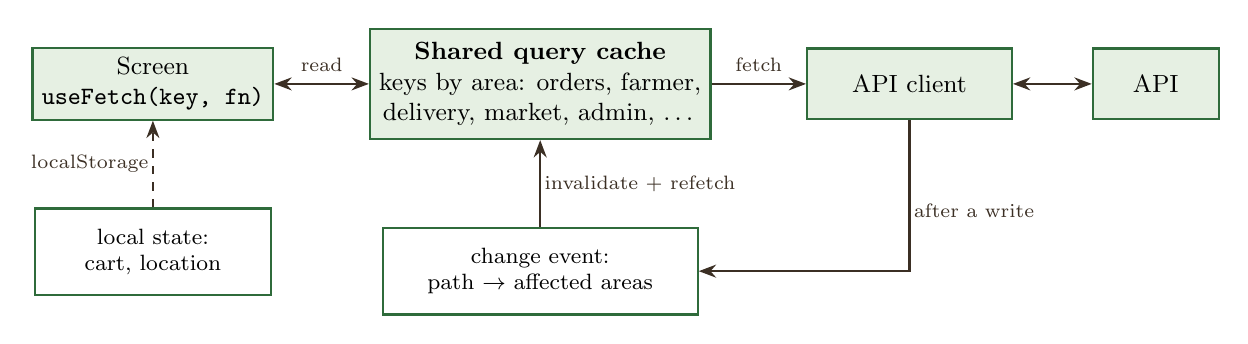
\begin{tikzpicture}[node distance=7mm and 12mm]
  \node[box, minimum width=30mm] (screen) {Screen\\\texttt{useFetch(key, fn)}};
  \node[box, right=of screen, minimum width=40mm, minimum height=14mm] (cache) {\textbf{Shared query cache}\\keys by area: orders, farmer,\\delivery, market, admin, \dots};
  \node[box, right=of cache, minimum width=26mm] (client) {API client};
  \node[box, right=10mm of client, minimum width=16mm] (api) {API};
  \node[sbox, below=11mm of cache, minimum width=40mm, minimum height=11mm] (bus) {change event:\\path $\to$ affected areas};
  \node[sbox, below=11mm of screen, minimum width=30mm, minimum height=11mm] (local) {local state:\\cart, location};
  \draw[darr] (screen) -- node[lbl,above=1mm]{read} (cache);
  \draw[arr] (cache) -- node[lbl,above=1mm]{fetch} (client);
  \draw[darr] (client) -- (api);
  \draw[arr] (client.south) |- node[lbl,pos=0.3,right]{after a write} (bus.east);
  \draw[arr] (bus) -- node[lbl,right]{invalidate + refetch} (cache);
  \draw[arr, dashed] (local) -- node[lbl,left]{localStorage} (screen);
\end{tikzpicture}}
\caption{Client data flow: every write announces its path and the cache refreshes every affected screen.}
\label{fig:clientdata}
\Description{Screens read from a shared query cache, which fetches through the API client. After a write, a change event maps the path to areas, which are invalidated and refetched. The cart and location are local state.}
\end{figure}

\begin{figure}[H]
  \centering
  \fbox{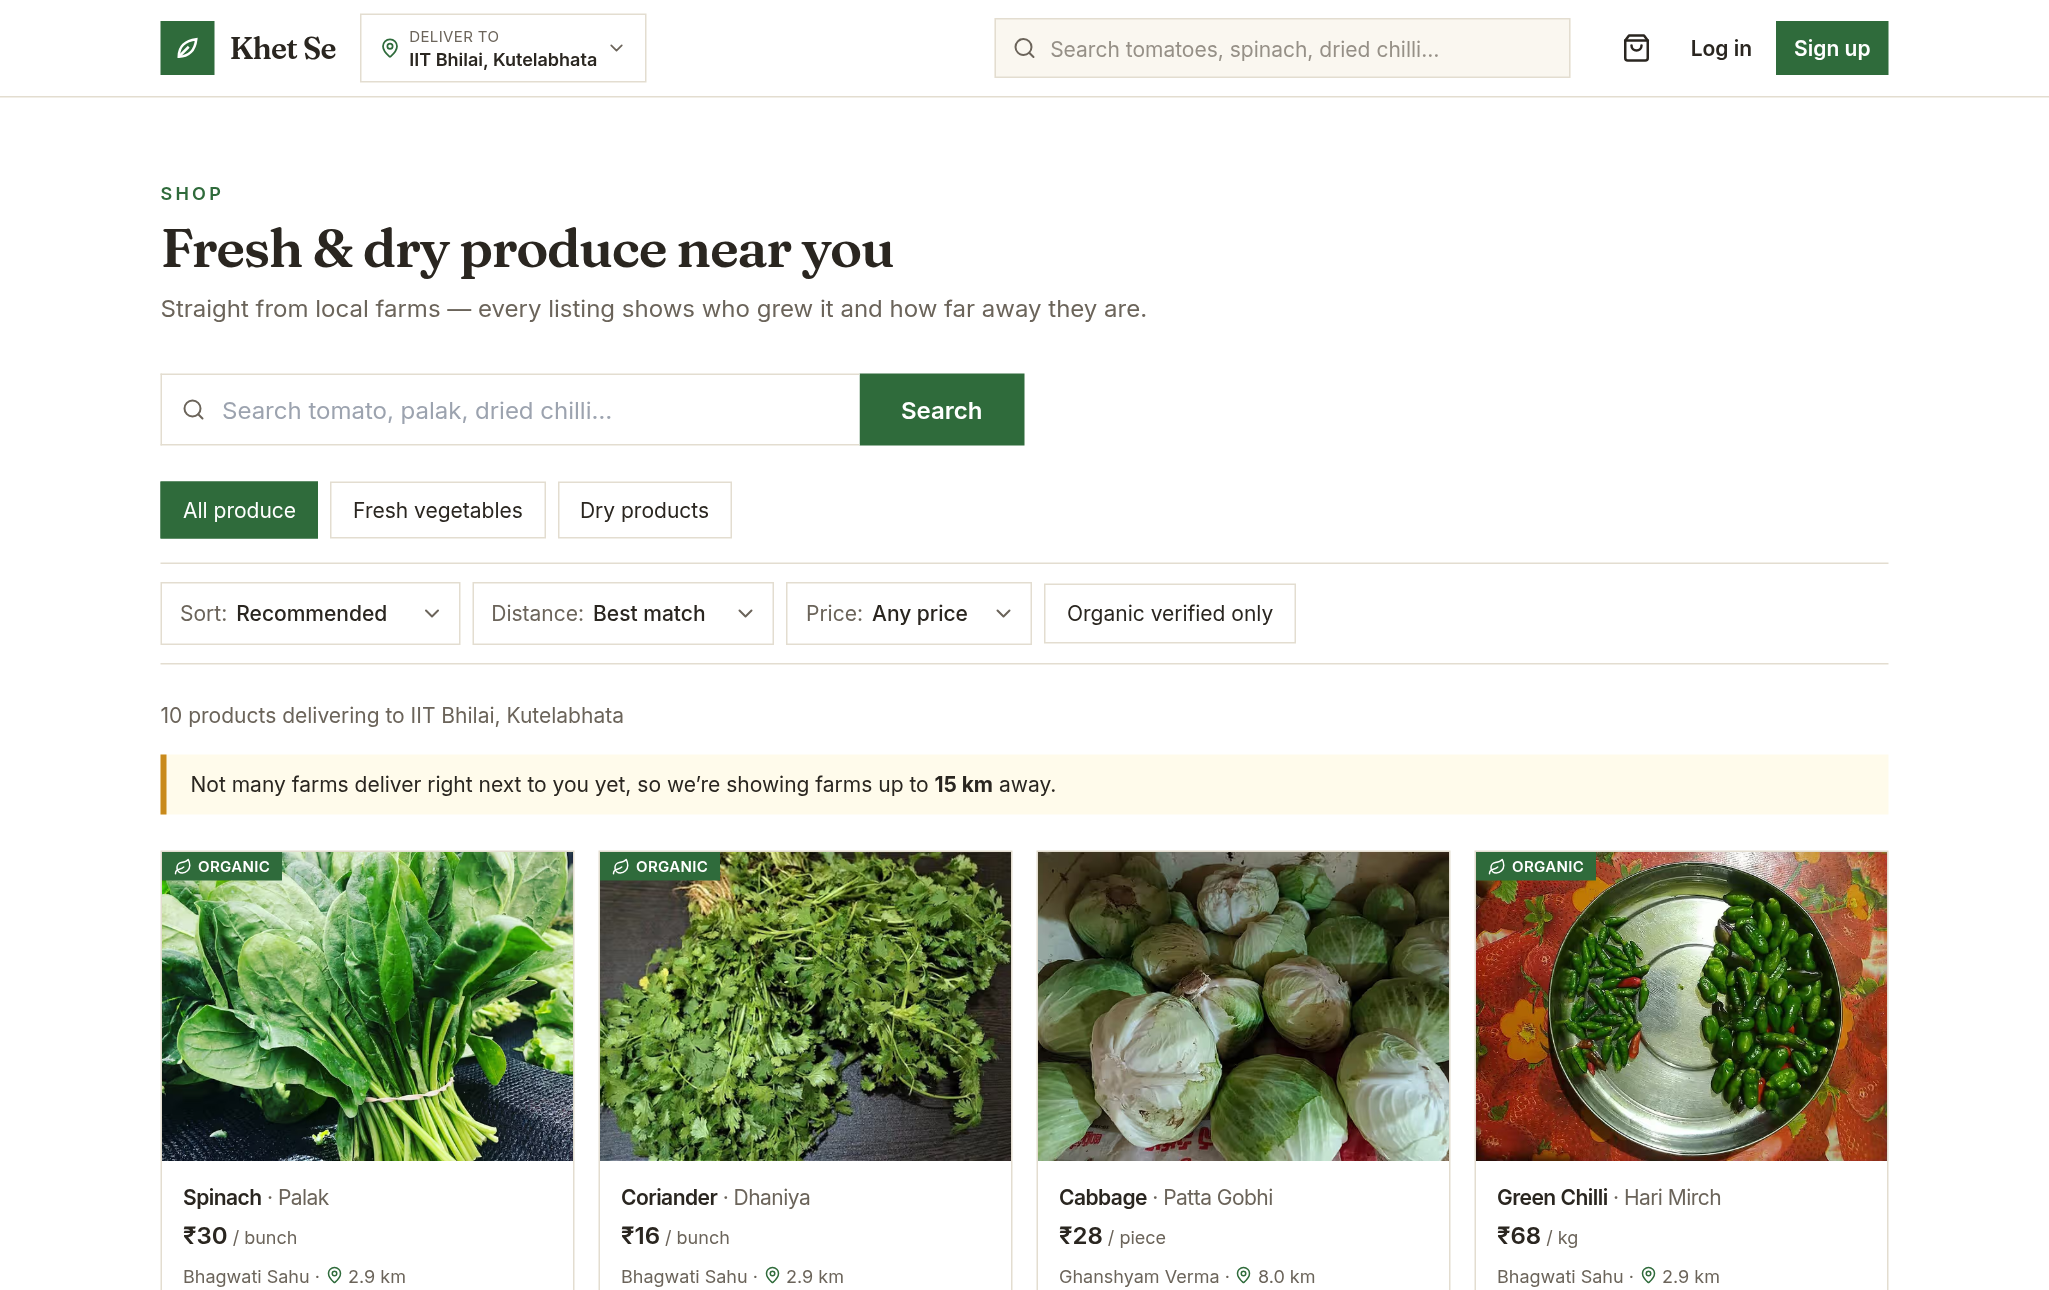
\includegraphics[width=0.92\linewidth]{03-shop}}
  \caption{Application interface: the shop lists every listing that delivers to the customer's location, with search, type, distance, price and organic filters.}
  \label{fig:ui}
  \Description{Shop page with a filter bar and a grid of product cards showing farm, distance, price and freshness.}
\end{figure}

\subsubsection*{Customer} Screens used by shoppers and guests, from discovery to order tracking.
\shot{01-home}{Home page with search, produce categories and the delivery location in the header.}{Home page with a search box, category tiles and a location selector.}
\shot{02-home-nearby}{``Farmers near you'': ranked farms with distance, organic verification, rating and starting prices.}{Cards of nearby farms with distance, badges and ratings.}
\shot{04-product}{Product page: price, freshness, a delivery check for this address, the farmer and farm, and the same product from other farms.}{Product page with price, freshness, delivery availability and farm information.}
\shot{05-farmer-profile}{Public farmer profile with story, practices, farms on a map and products in stock.}{Farmer profile page with a map and product list.}
\shot{08-cart}{Cart grouped by farm and priced live by the server, with a delivery fee per farm and the free-delivery threshold.}{Cart with items grouped by farm and per-farm delivery fees.}
\shot{09-checkout}{Checkout: saved address, payment method and the server-checked order summary.}{Checkout with address, payment method and order summary.}
\shot{11-order-tracking}{Order tracking: per-farm progress, the 4-digit delivery code and the delivery partner on the way.}{Order page with per-farm progress, delivery code and partner details.}

\begin{figure}[H]\centering
\begin{subfigure}{0.48\linewidth}\centering\fbox{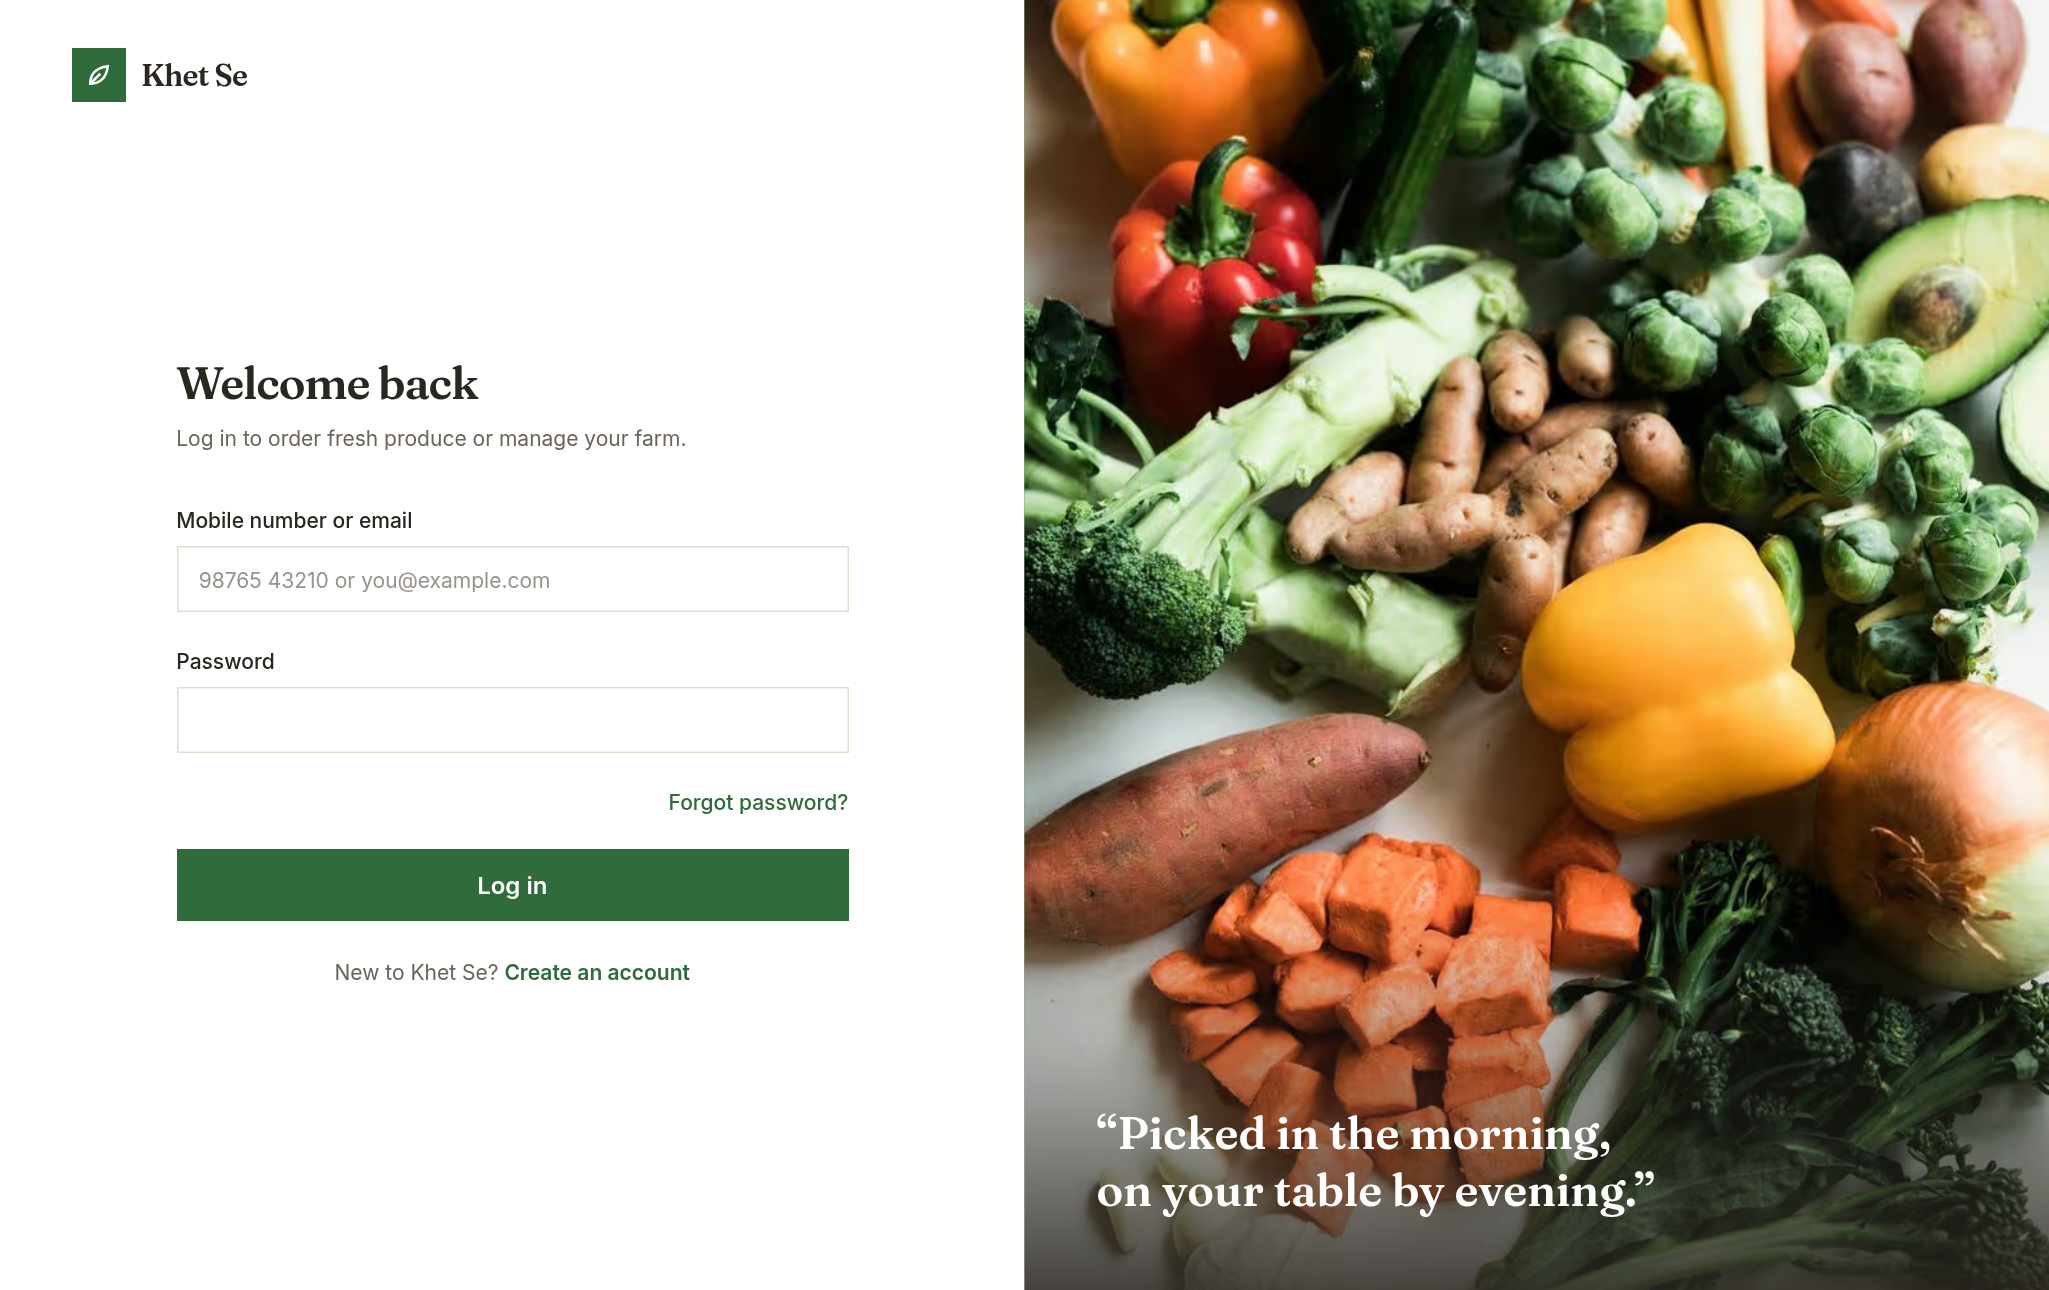
\includegraphics[width=0.96\linewidth]{06-login}}\caption{Login with mobile number or email.}\end{subfigure}\hfill
\begin{subfigure}{0.48\linewidth}\centering\fbox{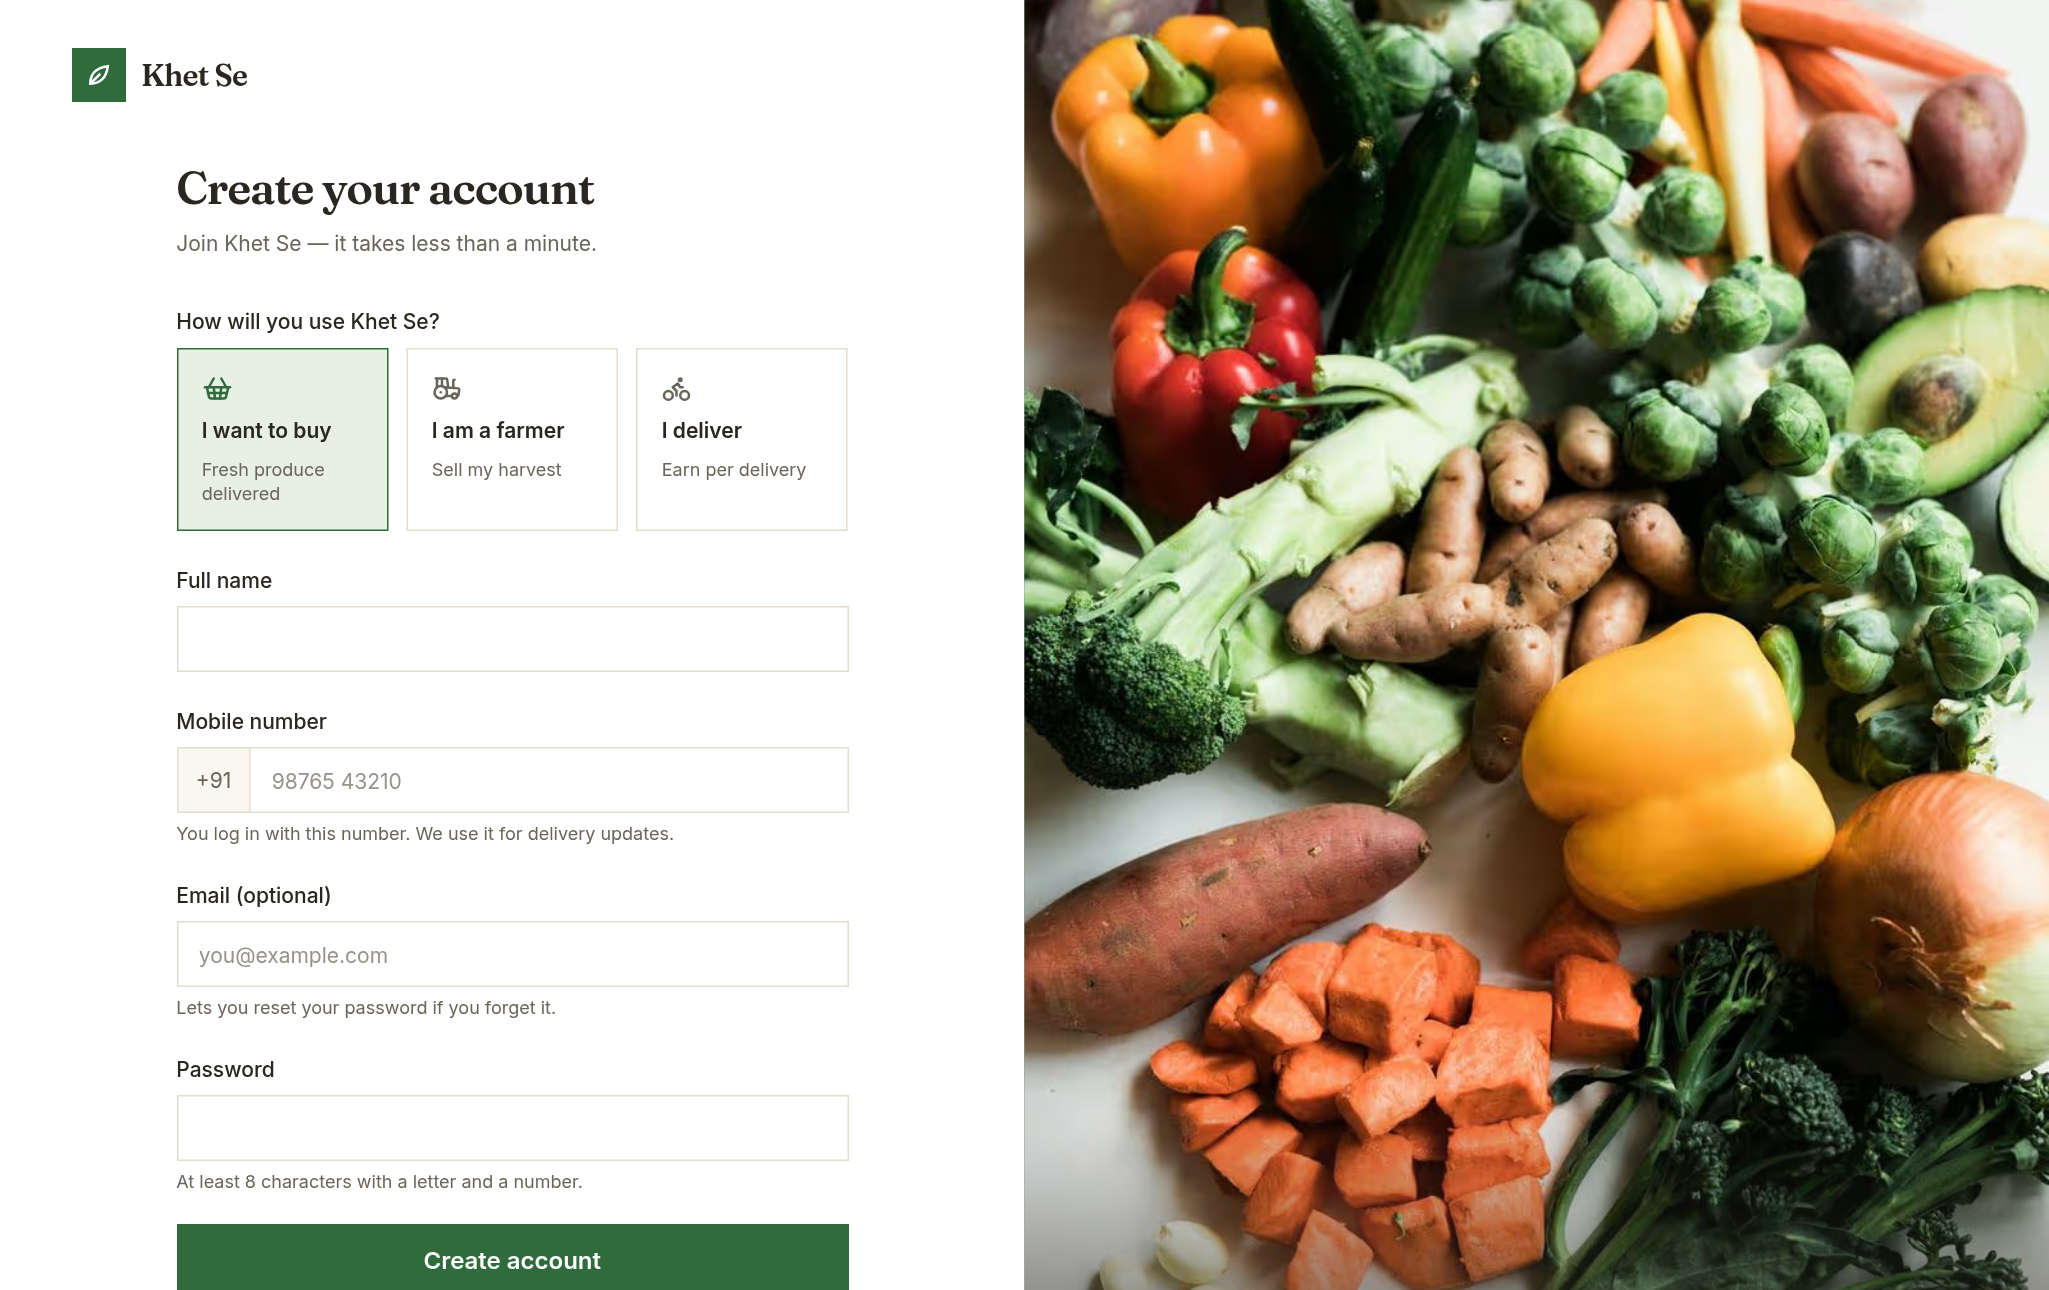
\includegraphics[width=0.96\linewidth]{07-register}}\caption{Sign-up with role choice; email optional.}\end{subfigure}
\caption{Authentication screens.}
\label{fig:authscreens}
\Description{Login form with mobile or email and password, and a registration form with name, mobile, optional email, password and role.}
\end{figure}

\subsubsection*{Farmer} The farmer dashboard, used mostly on phones.
\shot{12-farmer-overview}{Farmer dashboard: set-up checklist, orders to deliver, products on sale, stock warnings and verification status.}{Farmer dashboard with summary counts and checklist.}
\shot{13-farmer-orders}{Incoming orders with address, distance, acceptance deadline and the choice to deliver personally or request a partner.}{List of incoming orders with actions.}
\shot{14-farmer-to-deliver}{Orders to deliver, showing which partner is collecting or on the way.}{Orders ready for delivery with partner status.}
\shot{15-farmer-inventory}{Inventory with stock levels, quick stock edits and status filters.}{Inventory table with stock and status.}

\subsubsection*{Delivery partner} The partner dashboard: overview, job board and active jobs.
\shot{16-partner-overview}{Partner overview: online switch, earnings, distance, cash collected and active jobs.}{Partner dashboard with online toggle and earnings.}
\shot{17-partner-board}{Job board: open deliveries in the work area with pay, trip length, pickup distance and cash to collect; contacts appear only after accepting.}{List of open delivery jobs with pay and distances.}
\shot{18-partner-active}{Active deliveries: call and directions for pickup and drop, then handover with the customer's code.}{Active jobs with pickup and drop actions.}

\subsubsection*{Administrator} The admin console for verification, people, orders, refunds and audit.
\shot{19-admin-overview}{Admin overview: farmers to verify, orders waiting, jobs without a partner, refunds owed and business numbers.}{Admin dashboard with attention items and metrics.}
\shot{20-admin-verification}{Farmer verification: details, farms, certificate and decisions; a rejection requires a reason that the farmer sees.}{Verification cards with verify and reject buttons.}
\shot{21-admin-orders}{Orders with status, payment and refund filters and search by order number, name or mobile.}{Admin order list with filters.}
\shot{22-admin-order-detail}{Order detail for support: each farm's part, history, partner and payout, payments, refunds and admin history.}{Detailed order view for administrators.}
\shot{23-admin-people}{People: search and filter customers, farmers, partners and admins; suspend or reactivate.}{People list with role filters.}
\shot{24-admin-audit}{Audit trail: every admin decision with who, what, when and why.}{Audit log table.}

\begin{figure}[H]\centering
\begin{subfigure}{0.32\linewidth}\centering\fbox{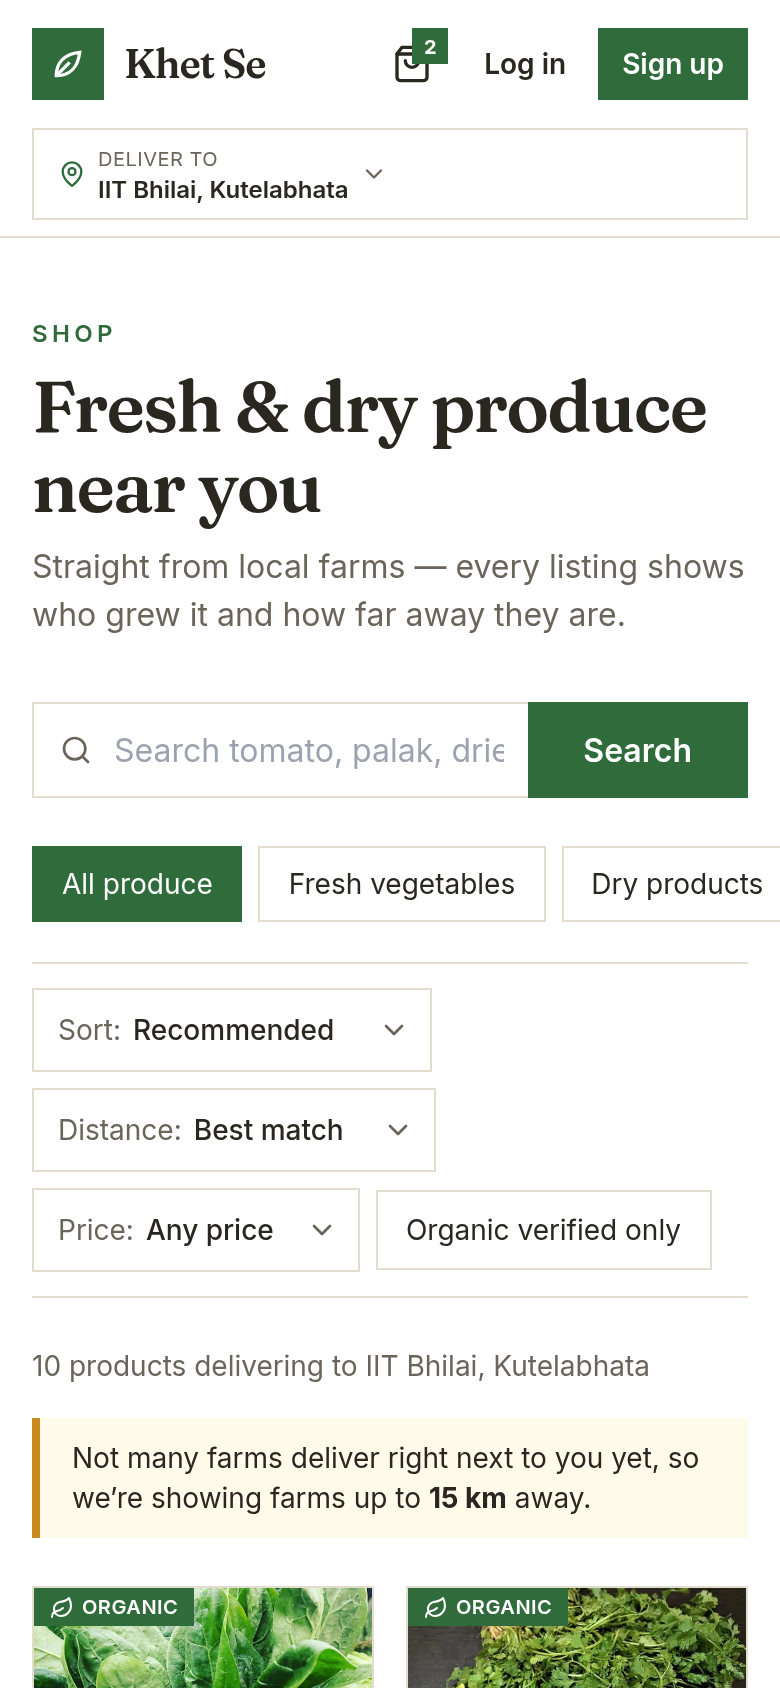
\includegraphics[width=0.95\linewidth]{25-mobile-shop}}\caption{Shop.}\end{subfigure}\hspace{8mm}
\begin{subfigure}{0.32\linewidth}\centering\fbox{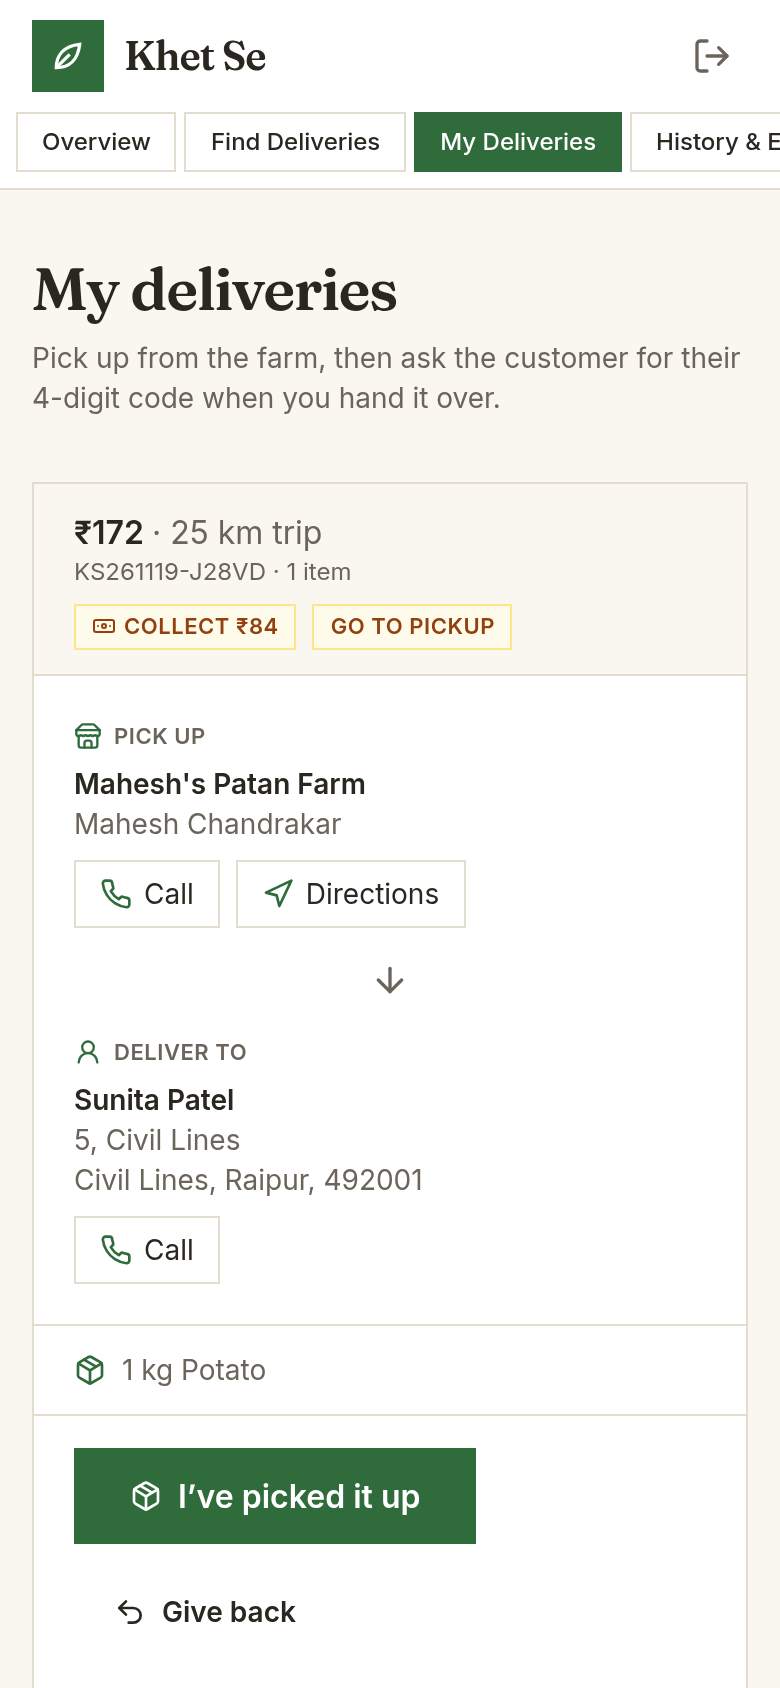
\includegraphics[width=0.95\linewidth]{26-mobile-partner}}\caption{Partner's active deliveries.}\end{subfigure}
\caption{Mobile layouts, the primary devices for farmers and partners.}
\label{fig:mobile}
\Description{Two phone screenshots: the shop and the partner's active deliveries.}
\end{figure}

\subsection{Database and Storage}
\label{sec:storage}

\begin{figure}[H]\centering
\fitbox{%
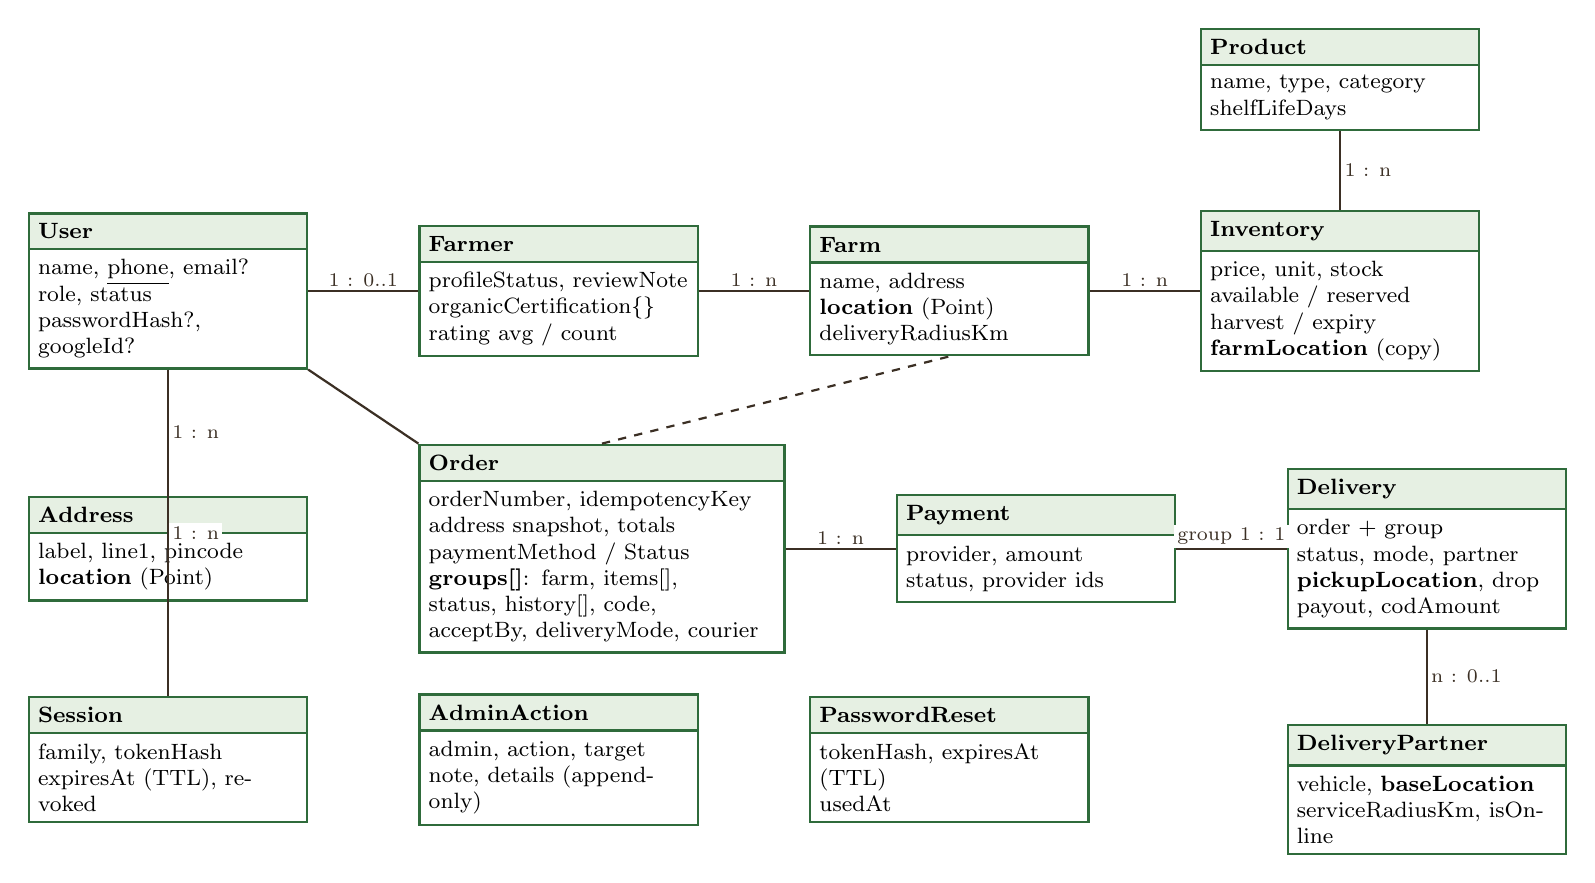
\begin{tikzpicture}[node distance=10mm and 14mm,
  ent/.style={draw=leaf, thick, rectangle split, rectangle split parts=2, rectangle split part fill={leafl,white}, font=\footnotesize, align=left, minimum width=34mm, text width=33mm},
  rel/.style={thick, color=soil}]
  \node[ent] (user) {\textbf{User}\nodepart{two}name, \underline{phone}, email?\\role, status\\passwordHash?, googleId?};
  \node[ent, right=of user] (farmer) {\textbf{Farmer}\nodepart{two}profileStatus, reviewNote\\organicCertification\{\}\\rating avg / count};
  \node[ent, right=of farmer] (farm) {\textbf{Farm}\nodepart{two}name, address\\\textbf{location} (Point)\\deliveryRadiusKm};
  \node[ent, right=of farm] (inv) {\textbf{Inventory}\nodepart{two}price, unit, stock\\available / reserved\\harvest / expiry\\\textbf{farmLocation} (copy)};
  \node[ent, above=of inv] (prod) {\textbf{Product}\nodepart{two}name, type, category\\shelfLifeDays};
  \node[ent, below=16mm of user] (addr) {\textbf{Address}\nodepart{two}label, line1, pincode\\\textbf{location} (Point)};
  \node[ent, right=of addr, text width=44mm, minimum width=45mm] (order) {\textbf{Order}\nodepart{two}orderNumber, idempotencyKey\\address snapshot, totals\\paymentMethod / Status\\\textbf{groups[]}: farm, items[],\\status, history[], code,\\acceptBy, deliveryMode, courier};
  \node[ent, right=of order] (pay) {\textbf{Payment}\nodepart{two}provider, amount\\status, provider ids};
  \node[ent, right=of pay] (del) {\textbf{Delivery}\nodepart{two}order + group\\status, mode, partner\\\textbf{pickupLocation}, drop\\payout, codAmount};
  \node[ent, below=12mm of del] (dp) {\textbf{DeliveryPartner}\nodepart{two}vehicle, \textbf{baseLocation}\\serviceRadiusKm, isOnline};
  \node[ent, below=12mm of addr] (sess) {\textbf{Session}\nodepart{two}family, tokenHash\\expiresAt (TTL), revoked};
  \node[ent, right=of sess] (aa) {\textbf{AdminAction}\nodepart{two}admin, action, target\\note, details (append-only)};
  \node[ent, right=of aa] (pr) {\textbf{PasswordReset}\nodepart{two}tokenHash, expiresAt (TTL)\\usedAt};
  \draw[rel] (user) -- node[lbl,above]{1 : 0..1} (farmer);
  \draw[rel] (farmer) -- node[lbl,above]{1 : n} (farm);
  \draw[rel] (farm) -- node[lbl,above]{1 : n} (inv);
  \draw[rel] (prod) -- node[lbl,right]{1 : n} (inv);
  \draw[rel] (user) -- node[lbl,right]{1 : n} (addr);
  \draw[rel] (user.south east) -- (order.north west);
  \draw[rel] (order) -- node[lbl,above]{1 : n} (pay);
  \draw[rel] (pay) -- node[lbl,above]{group 1 : 1} (del);
  \draw[rel] (del) -- node[lbl,right]{n : 0..1} (dp);
  \draw[rel, dashed] (order.north) -- (farm.south);
  \draw[rel] (user) -- node[lbl,right]{1 : n} (sess);
\end{tikzpicture}}
\caption{Data model (MongoDB collections). Points are GeoJSON with 2dsphere indexes.}
\label{fig:er}
\Description{Entity diagram of User, Farmer, Farm, Inventory, Product, Address, Order with embedded groups, Payment, Delivery, DeliveryPartner, Session, AdminAction and PasswordReset with their cardinalities.}
\end{figure}

\paragraph{Embedding versus referencing.} An order's farm parts, item snapshots, status history and address snapshot are \emph{embedded}: they belong to the order, are bounded in size and must change atomically with it; item prices are snapshots, so later price edits never alter past orders. Listings, farms, payments, deliveries and sessions are \emph{referenced}: they grow without bound, are queried on their own or have their own life cycle. \texttt{Inventory.farmLocation} is a \emph{denormalised copy} of the farm's point, so one \texttt{\$geoNear} over listings needs no join; it is re-synced whenever a farm moves and verified by the algorithm checker.

\begin{table}[htbp]
  \caption{Principal indexes}
  \label{tab:indexes}
  \small
  \begin{tabularx}{\columnwidth}{@{}p{0.2\columnwidth}p{0.38\columnwidth}L@{}}
    \toprule
    \textbf{Collection} & \textbf{Index} & \textbf{Serves} \\
    \midrule
    inventory & \texttt{farmLocation: 2dsphere} & product discovery \\
    farms & \texttt{location: 2dsphere} & farm discovery, checkout distances \\
    deliveries & \texttt{pickupLocation: 2dsphere, status} & partner job board \\
    deliveries & \texttt{partner, status, updatedAt} & a partner's own jobs \\
    orders & \texttt{customer, idempotencyKey} (unique) & duplicate-submission protection \\
    orders & \texttt{groups.farmer, groups.status, createdAt} & farmer queues \\
    orders & \texttt{groups.status, groups.acceptBy} & acceptance-deadline job \\
    users & \texttt{phone}, \texttt{email} (unique, partial) & login by mobile or email \\
    sessions, resets & \texttt{expiresAt} (TTL) & automatic clean-up \\
    \bottomrule
  \end{tabularx}
\end{table}

\paragraph{Insert, update, retrieve, maintain.} Writes go through services, using conditional updates or transactions as described in Section~\ref{sec:architecture}. Reads use index-backed queries with projections and cursor-free pagination by page and limit. Indexes are declared in the models and synchronised by a script on every deployment. TTL indexes remove expired sessions and reset tokens automatically. Configuration and secrets are environment variables, validated at start-up by a schema so a misconfigured server refuses to start. Uploaded images are restricted by type and size. At about 3\,KB per order, one city produces roughly 1\,GB of order data per year.

%% =====================================================================
\section{CSD Themes and Topics Applied in the Project}
\label{sec:csd-themes}

Table~\ref{tab:csd-themes} maps the system design themes to the components where they were applied and the reasons for each choice. Themes that are prepared for but not yet active are stated as such. \aiuse

\begin{table*}[t]
  \caption{Mapping of relevant themes and topics to their use in the project}
  \label{tab:csd-themes}
  \footnotesize
  \setlength{\tabcolsep}{5pt}
  \renewcommand{\arraystretch}{1.25}

  \begin{tabularx}{\textwidth}{@{}
    p{0.17\textwidth}
    p{0.27\textwidth}
    X
    @{}}
    \toprule
    \textbf{Theme / Topic} &
    \textbf{Where Used in the Project} &
    \textbf{Justification / Design Rationale} \\
    \midrule

    API Design &
    REST API under \texttt{/api}; one JSON envelope; Zod schemas; Idempotency-Key on checkout &
    Resource paths and standard status codes make the API usable by any client; 409 for conflicts lets clients react (``job taken'', ``price changed''); idempotency makes retries safe on poor mobile networks. \\

    Load Balancing &
    Not active at launch; stateless API, Redis-ready cache and rate limits &
    One process serves about $45\times$ the launch peak, so a balancer would add cost without benefit. Because no state lives in the process, adding processes behind a round-robin balancer (pm2 cluster mode or a reverse proxy) is a configuration change. \\

    Caching &
    Client query cache; 60\,s discovery result cache; catalogue cache; HTTP ETags; geocoding cache &
    Discovery is the most expensive read and tolerates a minute of staleness; caches are invalidated on any change that affects results, so correctness-critical paths (checkout) always read the database. \\

    Database Indexing / Query Optimization &
    2dsphere indexes; compound indexes for queues and jobs; partial unique and TTL indexes; batched \texttt{\$in} joins &
    \texttt{\$geoNear} is $O(\log n + k)$; batching replaced about 3{,}000 lookups per request with three; polling screens are index-only, keeping them under 20\,ms. \\

    Concurrency / Asynchronous Processing &
    Conditional atomic updates; multi-document transactions; non-blocking Node.js I/O; background jobs; email sent in the background &
    Correctness under races without application locks; scheduled jobs release abandoned stock and reconcile payments without blocking requests. \\

    Microservices vs. Monolith &
    Modular monolith: one API with ten modules &
    Checkout needs a local ACID transaction across modules; microservices would require sagas and extra operations. Module ownership of collections keeps later extraction possible. \\

    Design Patterns &
    Layered architecture; middleware chain (chain of responsibility); state machine; adapter/strategy for email and payment providers; observer-style change events; shared query-cache singleton &
    Each pattern isolates one concern: transport, business rules, provider choice, or UI refresh, so each can change or be tested alone. \\

    Authentication / Authorization &
    JWT access tokens, rotating refresh sessions, Google OAuth (PKCE), role middleware, ownership checks in services &
    Short-lived stateless tokens keep requests cheap; server-side refresh sessions allow revocation and theft detection; roles enforce strict data boundaries between four user types. \\

    Containerization / Deployment &
    Dockerfiles built in CI; production on pm2 with a self-contained runtime &
    The target server allows neither root nor Docker for the service account, so supervision with pm2 gives restart and logging; images remain ready for container hosts. \\

    Error Handling and Resilience &
    Typed \texttt{ApiError}s; central handler; rate limits; graceful shutdown; fallbacks for external services; reconciliation and stock-audit jobs &
    Clients get predictable errors; external outages degrade features rather than fail requests; safety-net jobs detect and repair drift. \\

    Algorithms and Complexity &
    Geo retrieval, adaptive radius, weighted scoring, Bayesian rating, diversity re-rank, first-wins matching &
    Chosen for explainability and bounded cost ($O(k)$ or $O(k\,m)$ per request) with no training data required at launch. \\

    Testing Strategy &
    Unit, 138 integration tests, role journeys, independent algorithm oracle (3{,}469 checks), workload model &
    Integration tests use a real replica set so transactions and races are tested; the oracle re-implements the rules independently and found four defects. \\

    Version Control / CI-CD &
    Git with separate client and server repositories on GitHub; GitHub Actions; one-command server update &
    Every push is typechecked, tested and built; deployment is repeatable (pull, build, sync indexes, reload). \\

    \bottomrule
  \end{tabularx}
\end{table*}

\paragraph{Modular monolith versus microservices.} The decisive factor was the checkout transaction. Reserving stock across several listings, writing the order and recording payment must be atomic. Inside one process with a replica set this is a short transaction that MongoDB guarantees. As microservices, it would require a saga with compensations for every failure point and an outbox for reliable messaging, more infrastructure than the whole launch deployment. We kept the benefits that matter at this stage, clear ownership and independent testability, through module boundaries and a layered structure, and measured that one process has ample headroom.

\paragraph{Concurrency control by conditional updates.} The alternatives were pessimistic locks (serialising every checkout or claim), optimistic read-modify-write with retries (more code and more round trips), or a queue that processes orders one by one (added latency and infrastructure). Expressing each invariant as a filter on a single atomic update makes the database the arbiter: the second of two racing buyers or partners simply matches nothing and receives a clear 409. Only checkout, which spans several documents, uses a transaction.

\paragraph{Geo-indexed discovery with caching.} Location drives every customer query, so it must be served by an index, not by computing distances in application code. Combining \texttt{\$geoNear} with batched joins and a short result cache keeps discovery fast; invalidating the cache on every relevant change and never caching checkout keeps it correct. The single shared sellability rule removed the inconsistency between what search shows and what checkout accepts.

%% =====================================================================
\section{Results and Evaluation}
\label{sec:results}

\paragraph{Correctness.} The first run of the independent algorithm checker found four defects, all of which were fixed and covered by regression tests (Table~\ref{tab:defects}). After the fixes, all 3{,}469 checks pass (Figure~\ref{fig:results}). All 138 API integration tests pass locally, in CI and on the deployment server.

\begin{table}[htbp]
  \caption{Defects found by the independent algorithm checker}
  \label{tab:defects}
  \small
  \begin{tabularx}{\columnwidth}{@{}Lp{0.36\columnwidth}@{}}
    \toprule
    \textbf{Defect} & \textbf{Fix} \\
    \midrule
    Expired dry goods and produce past its shelf life were offered and could be ordered. & Shared sellability rule in every path. \\
    A listing with less stock than one minimum order was shown but could never be ordered. & Search requires stock $\ge$ minimum order. \\
    Checkout rounded the distance before comparing it with the delivery radius, accepting at 3.00--3.05\,km what search hid. & Exact comparison; rounding only for display and fees. \\
    Price scores were skewed by the expired items. & Resolved by the first fix. \\
    \bottomrule
  \end{tabularx}
\end{table}

\begin{figure}[H]
  \centering
  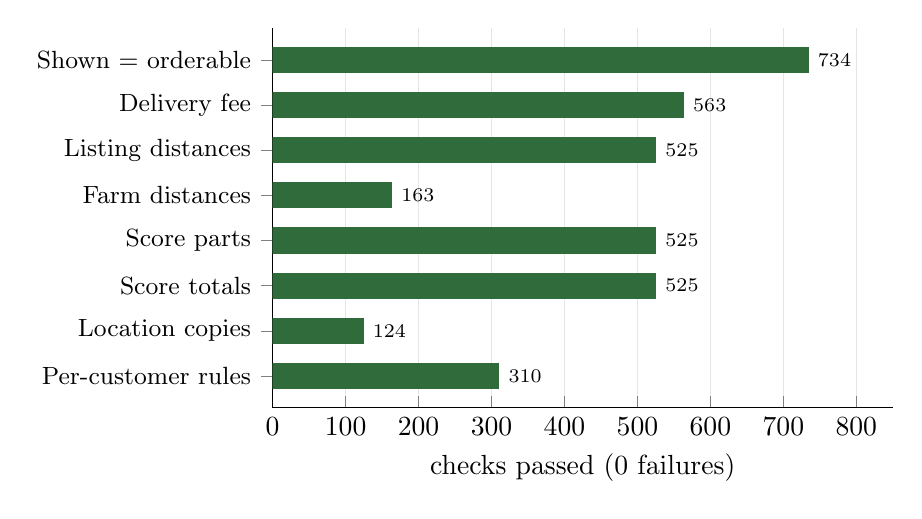
\begin{tikzpicture}
  \begin{axis}[
    xbar, width=0.78\linewidth, height=6.4cm,
    xmin=0, xmax=850,
    xlabel={checks passed (0 failures)},
    symbolic y coords={{Per-customer rules},{Location copies},{Score totals},{Score parts},{Farm distances},{Listing distances},{Delivery fee},{Shown = orderable}},
    ytick=data, yticklabel style={font=\small},
    nodes near coords, nodes near coords style={font=\scriptsize},
    bar width=3.2mm, axis lines*=left, xmajorgrids, grid style={gray!20},
  ]
  \addplot[fill=leaf, draw=leaf] coordinates {(310,{Per-customer rules}) (124,{Location copies}) (525,{Score totals}) (525,{Score parts}) (163,{Farm distances}) (525,{Listing distances}) (563,{Delivery fee}) (734,{Shown = orderable})};
  \end{axis}
  \end{tikzpicture}
  \caption{Representative results: independent algorithm verification on the Durg--Bhilai test bed after the fixes, 3{,}469 checks with no failures. ``Per-customer rules'' covers eligibility, radius widening, five sort orders, diversity and filters for each of the 27 customers.}
  \label{fig:results}
  \Description{Horizontal bar chart of passed checks: shown equals orderable 734, delivery fee 563, listing distances 525, farm distances 163, score parts 525, score totals 525, location copies 124, per-customer rules 310.}
\end{figure}

\paragraph{Functional outcomes.} Every requirement in Table~\ref{tab:requirements} is implemented and demonstrated in the screenshots of Section~\ref{sec:frontend}. The race tests confirm the correctness requirements: six buyers racing for three units sell exactly three; two partners accepting one job produce one assignment and one 409; repeated checkout submissions with one key create one order; a replayed refresh token revokes its family (43 of 43 replays detected during load testing).

\subsection{Performance}
\label{sec:performance}

\paragraph{Setup.} A workload generator simulates the three populations together against a production build with one API process. Customers arrive as a Poisson process at 18.7 sessions per minute times a multiplier, with a mix of 62.5\% browse, 10\% abandoned cart, 12.5\% purchase and 15\% order tracking. 200 farmers check their queues every 60--120\,s and accept, pack, deliver or request a partner; 60 partners refresh the board every 15--25\,s, then claim, pick up and hand over. Every simulated person has its own client IP, so real rate limits apply, and uses real token refresh. Think and travel times are compressed; arrival rates are not.

\begin{table}[htbp]
  \caption{Launch peak and stress results (one API process)}
  \label{tab:perf}
  \small
  \begin{tabular}{@{}lrrrrr@{}}
    \toprule
    \textbf{Profile} & \textbf{req/s} & \textbf{Reads p95} & \textbf{Writes p95} & \textbf{Errors} & \textbf{API CPU} \\
    \midrule
    Launch peak (1$\times$, 5 min) & 13.3 & 20\,ms & 31\,ms & 0 & 12\% \\
    Stress (3$\times$, 3 min) & 17.0 & 28\,ms & 33\,ms & 0 & 16\% \\
    \bottomrule
  \end{tabular}
\end{table}

\begin{figure}[H]\centering
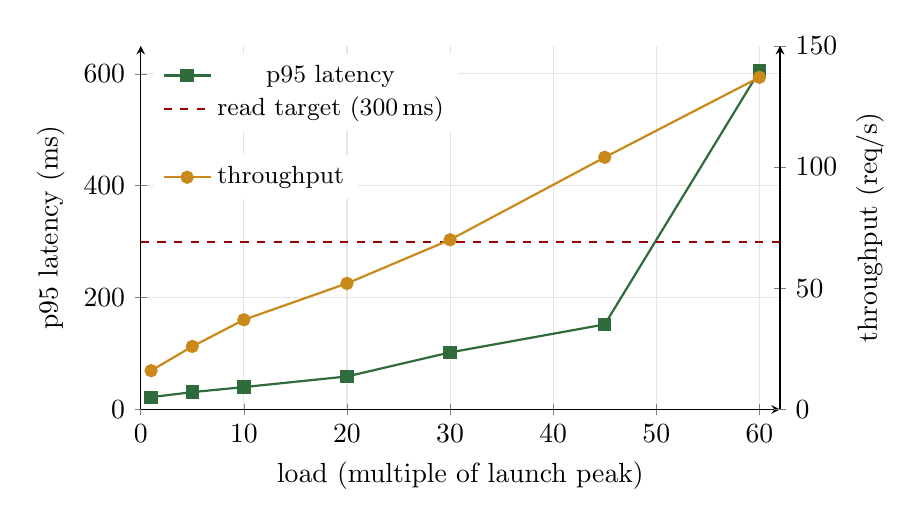
\begin{tikzpicture}
\begin{axis}[
  width=0.8\linewidth, height=6.2cm,
  xlabel={load (multiple of launch peak)}, ylabel={p95 latency (ms)},
  xmin=0, xmax=62, ymin=0, ymax=650,
  grid=major, grid style={gray!20},
  axis lines=left, legend style={at={(0.02,0.98)}, anchor=north west, font=\small, draw=none},
  every axis plot/.append style={thick},
]
\addplot[color=leaf, mark=square*] coordinates {(1,22) (5,31) (10,40) (20,59) (30,102) (45,152) (60,605)};
\addlegendentry{p95 latency}
\addplot[color=red!60!black, dashed, domain=0:62] {300};
\addlegendentry{read target (300\,ms)}
\end{axis}
\begin{axis}[
  width=0.8\linewidth, height=6.2cm,
  xmin=0, xmax=62, ymin=0, ymax=150,
  axis y line=right, axis x line=none, ylabel={throughput (req/s)},
  legend style={at={(0.02,0.70)}, anchor=north west, font=\small, draw=none},
]
\addplot[color=turmeric, mark=*, thick] coordinates {(1,16) (5,26) (10,37) (20,52) (30,70) (45,104) (60,137)};
\addlegendentry{throughput}
\end{axis}
\end{tikzpicture}
\caption{Capacity ramp of one API process. Latency stays within the target up to about $45\times$ the launch peak ($\approx$104\,req/s); at $60\times$ the single JavaScript core saturates and $p95$ rises to 605\,ms.}
\label{fig:capacity}
\Description{Line chart: p95 latency rises from 22 ms at 1x to 152 ms at 45x and 605 ms at 60x, crossing the 300 ms target between 45x and 60x; throughput rises from 16 to 137 requests per second.}
\end{figure}

\paragraph{Findings.}
\begin{itemize}
  \item \textbf{Headroom.} One process serves about $45\times$ the expected launch peak; beyond that, more processes are needed, not a redesign.
  \item \textbf{Login is the costliest call.} Pure-JavaScript bcrypt blocks the event loop for about 230\,ms per login; 24 simultaneous logins took 5.7\,s each. Native bcrypt on the thread pool is the remedy.
  \item \textbf{Polling dominates steady traffic.} At launch peak about half of all requests are job-board refreshes and over a third are farmer queue checks; both are index-only and under 20\,ms.
  \item \textbf{Fleet size, not software, limits deliveries.} With realistic ride times (about 38 minutes per job), 60 partners just cover 98 jobs per hour; a $3\times$ peak needs about 184 partners or batched drops.
\end{itemize}

%% =====================================================================
\section{Discussion and Limitations}
\label{sec:discussion}

\paragraph{What worked well.} Expressing every invariant as a conditional update or a short transaction made the hardest requirements (no overselling, no double assignment, no duplicate orders) simple to implement and easy to test. The independent oracle was the most valuable validation step: it found defects that feature tests had not, because it compared the whole system against a separately written specification on realistic geography. The shared, self-invalidating client cache removed a class of stale-screen bugs that had appeared when each screen fetched its own data.

\paragraph{Limitations.}
\begin{itemize}
  \item \textbf{Synthetic data.} Ratings, orders and arrival patterns are modelled, not observed; ranking weights and capacity numbers must be re-checked with real usage.
  \item \textbf{Single machine.} The database is a one-member replica set on the same server as the application; a hardware failure stops the service, and backups are not yet automated.
  \item \textbf{Polling instead of push.} Simple and robust, but the largest share of steady traffic.
  \item \textbf{Self-selected jobs.} Fair and simple, but not route-optimal for dense demand.
  \item \textbf{In-process jobs and cache.} Correct for one process; several processes need Redis and a job queue so jobs run once.
  \item \textbf{Not yet enabled.} SMS verification of phone numbers, automatic refunds through the payment provider, HTTPS on a public domain and a configured email provider in production.
  \item \textbf{Straight-line distance} is used when road distance is unavailable, which underestimates trips across rivers or rail lines.
\end{itemize}

\paragraph{Future work.} Native bcrypt; a three-member replica set on separate machines with scheduled backups; server-sent events for queues and boards; Redis and a job queue for multiple API processes; batched and assisted dispatch; learning-to-rank once real interactions exist; native mobile applications using the same API; and per-city sharding for expansion.

%% =====================================================================
\section{AI Tool Usage Declaration}
\label{sec:ai-usage}

AI assistance was used extensively in this project. Claude Code (Anthropic's Claude models), used as a coding assistant in the terminal, generated most of the source code for the server and the client, the tests, the seed and workload scripts, the algorithm checker, the deployment scripts, the diagrams and the text of this report, under our direction. Every commit in both repositories was made with this assistance. Our own work was to define the problem and requirements, take the design decisions when alternatives were presented (for example, the delivery-partner role, a single-city launch, mobile-number login with optional email, and the shared query cache), test the application as customers, farmers, partners and administrators, report defects, provide and operate the deployment server, and review the results. AI-generated code was checked by running the automated test suite, the independent algorithm checker and the workload model, by manual testing of each role in the browser, and by reviewing the changes before committing and pushing them. We estimate that about 90\% of the project's code and documentation was produced with AI assistance. \aiuse

%% =====================================================================
\appendix

\section{Source Code and Repository}

The project consists of two Git repositories:
\begin{itemize}
  \item Server (API, scripts, tests, documentation and this report): \url{https://github.com/ashutosh-iitbhilai/khet-se-server}
  \item Client (web application): \url{https://github.com/ashutosh-iitbhilai/khet-se-client}
\end{itemize}

\paragraph{Server structure.} \texttt{src/routes}, \texttt{src/controllers}, \texttt{src/services} (including \texttt{recommendation/} and \texttt{order/}), \texttt{src/models}, \texttt{src/middleware}, \texttt{src/validators}, \texttt{src/jobs}, \texttt{src/config}, \texttt{src/scripts} (seeding, workload, algorithm checker, admin creation), \texttt{test/} (integration tests), \texttt{docs/} (architecture, deployment, audit, workload and algorithm-check documents, and \texttt{docs/report/}).

\paragraph{Client structure.} \texttt{app/} (App Router pages: \texttt{(shop)}, \texttt{(auth)}, \texttt{farmer}, \texttt{delivery}, \texttt{admin}), \texttt{features/} (role-specific components), \texttt{components/} (layout and UI primitives), \texttt{hooks/} (\texttt{useFetch}), \texttt{lib/} (API client, query client, configuration), \texttt{services/} (typed API calls).

\paragraph{Build and run.} With Node.js 20 and MongoDB (a replica set for transactions):
\begin{itemize}
  \item Server: \texttt{npm ci}; copy \texttt{.env.example} to \texttt{.env}; \texttt{npm run seed:catalogue}; \texttt{npm run seed:demo}; \texttt{npm run seed:activity}; \texttt{npm run dev}.
  \item Client: \texttt{npm ci}; set the API URL in \texttt{.env.local}; \texttt{npm run dev}.
  \item Tests: \texttt{npm test} (server). Algorithm check: \texttt{npm run seed:algo}, then \texttt{npm run algo:check}. Workload: \texttt{npm run workload -- setup}, \texttt{npm run workload -- run --profile peak}.
  \item Production: \texttt{npm run build}, then start both under pm2; the server's \texttt{update.sh} pulls, builds, synchronises indexes and reloads.
\end{itemize}

\end{document}
\endinput
